% Options for packages loaded elsewhere
\PassOptionsToPackage{unicode}{hyperref}
\PassOptionsToPackage{hyphens}{url}
%
\documentclass[
]{article}
\usepackage{amsmath,amssymb}
\usepackage{lmodern}
\usepackage{iftex}
\ifPDFTeX
  \usepackage[T1]{fontenc}
  \usepackage[utf8]{inputenc}
  \usepackage{textcomp} % provide euro and other symbols
\else % if luatex or xetex
  \usepackage{unicode-math}
  \defaultfontfeatures{Scale=MatchLowercase}
  \defaultfontfeatures[\rmfamily]{Ligatures=TeX,Scale=1}
\fi
% Use upquote if available, for straight quotes in verbatim environments
\IfFileExists{upquote.sty}{\usepackage{upquote}}{}
\IfFileExists{microtype.sty}{% use microtype if available
  \usepackage[]{microtype}
  \UseMicrotypeSet[protrusion]{basicmath} % disable protrusion for tt fonts
}{}
\makeatletter
\@ifundefined{KOMAClassName}{% if non-KOMA class
  \IfFileExists{parskip.sty}{%
    \usepackage{parskip}
  }{% else
    \setlength{\parindent}{0pt}
    \setlength{\parskip}{6pt plus 2pt minus 1pt}}
}{% if KOMA class
  \KOMAoptions{parskip=half}}
\makeatother
\usepackage{xcolor}
\usepackage{color}
\usepackage{fancyvrb}
\newcommand{\VerbBar}{|}
\newcommand{\VERB}{\Verb[commandchars=\\\{\}]}
\DefineVerbatimEnvironment{Highlighting}{Verbatim}{commandchars=\\\{\}}
% Add ',fontsize=\small' for more characters per line
\usepackage{framed}
\definecolor{shadecolor}{RGB}{248,248,248}
\newenvironment{Shaded}{\begin{snugshade}}{\end{snugshade}}
\newcommand{\AlertTok}[1]{\textcolor[rgb]{0.94,0.16,0.16}{#1}}
\newcommand{\AnnotationTok}[1]{\textcolor[rgb]{0.56,0.35,0.01}{\textbf{\textit{#1}}}}
\newcommand{\AttributeTok}[1]{\textcolor[rgb]{0.77,0.63,0.00}{#1}}
\newcommand{\BaseNTok}[1]{\textcolor[rgb]{0.00,0.00,0.81}{#1}}
\newcommand{\BuiltInTok}[1]{#1}
\newcommand{\CharTok}[1]{\textcolor[rgb]{0.31,0.60,0.02}{#1}}
\newcommand{\CommentTok}[1]{\textcolor[rgb]{0.56,0.35,0.01}{\textit{#1}}}
\newcommand{\CommentVarTok}[1]{\textcolor[rgb]{0.56,0.35,0.01}{\textbf{\textit{#1}}}}
\newcommand{\ConstantTok}[1]{\textcolor[rgb]{0.00,0.00,0.00}{#1}}
\newcommand{\ControlFlowTok}[1]{\textcolor[rgb]{0.13,0.29,0.53}{\textbf{#1}}}
\newcommand{\DataTypeTok}[1]{\textcolor[rgb]{0.13,0.29,0.53}{#1}}
\newcommand{\DecValTok}[1]{\textcolor[rgb]{0.00,0.00,0.81}{#1}}
\newcommand{\DocumentationTok}[1]{\textcolor[rgb]{0.56,0.35,0.01}{\textbf{\textit{#1}}}}
\newcommand{\ErrorTok}[1]{\textcolor[rgb]{0.64,0.00,0.00}{\textbf{#1}}}
\newcommand{\ExtensionTok}[1]{#1}
\newcommand{\FloatTok}[1]{\textcolor[rgb]{0.00,0.00,0.81}{#1}}
\newcommand{\FunctionTok}[1]{\textcolor[rgb]{0.00,0.00,0.00}{#1}}
\newcommand{\ImportTok}[1]{#1}
\newcommand{\InformationTok}[1]{\textcolor[rgb]{0.56,0.35,0.01}{\textbf{\textit{#1}}}}
\newcommand{\KeywordTok}[1]{\textcolor[rgb]{0.13,0.29,0.53}{\textbf{#1}}}
\newcommand{\NormalTok}[1]{#1}
\newcommand{\OperatorTok}[1]{\textcolor[rgb]{0.81,0.36,0.00}{\textbf{#1}}}
\newcommand{\OtherTok}[1]{\textcolor[rgb]{0.56,0.35,0.01}{#1}}
\newcommand{\PreprocessorTok}[1]{\textcolor[rgb]{0.56,0.35,0.01}{\textit{#1}}}
\newcommand{\RegionMarkerTok}[1]{#1}
\newcommand{\SpecialCharTok}[1]{\textcolor[rgb]{0.00,0.00,0.00}{#1}}
\newcommand{\SpecialStringTok}[1]{\textcolor[rgb]{0.31,0.60,0.02}{#1}}
\newcommand{\StringTok}[1]{\textcolor[rgb]{0.31,0.60,0.02}{#1}}
\newcommand{\VariableTok}[1]{\textcolor[rgb]{0.00,0.00,0.00}{#1}}
\newcommand{\VerbatimStringTok}[1]{\textcolor[rgb]{0.31,0.60,0.02}{#1}}
\newcommand{\WarningTok}[1]{\textcolor[rgb]{0.56,0.35,0.01}{\textbf{\textit{#1}}}}
\usepackage{longtable,booktabs,array}
\usepackage{calc} % for calculating minipage widths
% Correct order of tables after \paragraph or \subparagraph
\usepackage{etoolbox}
\makeatletter
\patchcmd\longtable{\par}{\if@noskipsec\mbox{}\fi\par}{}{}
\makeatother
% Allow footnotes in longtable head/foot
\IfFileExists{footnotehyper.sty}{\usepackage{footnotehyper}}{\usepackage{footnote}}
\makesavenoteenv{longtable}
\usepackage{graphicx}
\makeatletter
\def\maxwidth{\ifdim\Gin@nat@width>\linewidth\linewidth\else\Gin@nat@width\fi}
\def\maxheight{\ifdim\Gin@nat@height>\textheight\textheight\else\Gin@nat@height\fi}
\makeatother
% Scale images if necessary, so that they will not overflow the page
% margins by default, and it is still possible to overwrite the defaults
% using explicit options in \includegraphics[width, height, ...]{}
\setkeys{Gin}{width=\maxwidth,height=\maxheight,keepaspectratio}
% Set default figure placement to htbp
\makeatletter
\def\fps@figure{htbp}
\makeatother
\setlength{\emergencystretch}{3em} % prevent overfull lines
\providecommand{\tightlist}{%
  \setlength{\itemsep}{0pt}\setlength{\parskip}{0pt}}
\setcounter{secnumdepth}{-\maxdimen} % remove section numbering
% preamble used for exam
\usepackage{amsmath}
\usepackage{booktabs}
\usepackage{float}

\newcommand{\points}[1]
{\begin{flushright}\textbf{#1}\end{flushright}}
\newcommand{\solstart}
{\vspace{3ex}\textbf{Solution}:}
\newcommand{\solend}
{\vspace{2ex}$\blacksquare$}
\usepackage{booktabs}
\usepackage{longtable}
\usepackage{array}
\usepackage{multirow}
\usepackage{wrapfig}
\usepackage{float}
\usepackage{colortbl}
\usepackage{pdflscape}
\usepackage{tabu}
\usepackage{threeparttable}
\usepackage{threeparttablex}
\usepackage[normalem]{ulem}
\usepackage{makecell}
\usepackage{xcolor}
\ifLuaTeX
  \usepackage{selnolig}  % disable illegal ligatures
\fi
\IfFileExists{bookmark.sty}{\usepackage{bookmark}}{\usepackage{hyperref}}
\IfFileExists{xurl.sty}{\usepackage{xurl}}{} % add URL line breaks if available
\urlstyle{same} % disable monospaced font for URLs
\hypersetup{
  hidelinks,
  pdfcreator={LaTeX via pandoc}}

\author{}
\date{\vspace{-2.5em}}

\begin{document}

\thispagestyle{empty}

\begin{tabular}{l}
ETH Zurich \\
D-USYS\\
Institute of Agricultural Sciences\\
\end{tabular}

\vspace{15ex}
\begin{center}
\huge
Solutions To Exam\\ \vspace{1ex}
Livestock Breeding and Genomics \\  \vspace{1ex}
FS 2022 \\

\normalsize
\vspace{7ex}
Peter von Rohr 
\end{center}

\vspace{7ex}
\begin{tabular}{p{5cm}lr}
  & \textsc{Date}  & \textsc{\emph{23. December 2022}} \\
  & \textsc{Begin} & \textsc{\emph{09:15 }}\\
  & \textsc{End}   & \textsc{\emph{11:15 }}\\ 
\end{tabular}

\vspace{5ex}

\large
\begin{tabular}{p{2.5cm}p{3cm}p{6cm}}
  &  Name:     &  \\
  &            &  \\
  &  Legi-Nr:  & \\
\end{tabular}
\normalsize

\vspace{9ex}
\begin{center}
\begin{tabular}{|p{3cm}|c|c|}
\hline
Problem  &  Maximum Number of Points  &  Number of Points Reached \\
\hline
1        &  27         & \\
\hline
2        &  25         & \\
\hline
3        &  47         & \\
\hline
4        &  28          & \\
\hline
5        &  22          & \\
\hline
Total    &  149    & \\
\hline
\end{tabular}
\end{center}

\clearpage
\pagebreak

\hypertarget{problem-1-quantitative-genetics}{%
\subsection{Problem 1 Quantitative
Genetics}\label{problem-1-quantitative-genetics}}

The following dataset contains observations of a phenotypic trait and
genotypes for two loci. The numbers in the columns \texttt{SNP\_1} and
\texttt{SNP\_2} count the number of alleles with a positive effect on
the observation. Genotypic values of heterozygous animals are assumed to
be right between the genotypic values of homozygous animals (\(d=0\)).

\textit{Der folgende Datensatz enthält Beobachtungen für ein phänotypisches Merkmal und Genotypen von zwei Loci. Die Zahlen in den Kolonnen }
\verb+SNP_1+ \textit{ und } \verb+SNP_2+
\textit{ zählen die Anzahl Allele mit einem positiven Effekt auf den Merkmalswert. Genotypische Werte der heterozygoten Tiere sind genau in der Mitte zwischen den genotypischen Werten der homozygoten Tiere}
(\(d=0\)).

\begin{longtable}[]{@{}rrrr@{}}
\toprule()
Animal & SNP\_1 & SNP\_2 & Observation \\
\midrule()
\endhead
1 & 0 & 2 & 141 \\
2 & 0 & 1 & 120 \\
3 & 2 & 1 & 189 \\
4 & 1 & 2 & 172 \\
5 & 1 & 1 & 158 \\
6 & 1 & 1 & 152 \\
7 & 1 & 0 & 141 \\
8 & 0 & 1 & 116 \\
9 & 1 & 2 & 176 \\
10 & 0 & 0 & 107 \\
11 & 1 & 0 & 132 \\
12 & 1 & 2 & 173 \\
13 & 1 & 0 & 131 \\
14 & 0 & 2 & 144 \\
15 & 1 & 2 & 176 \\
16 & 1 & 2 & 175 \\
17 & 0 & 0 & 103 \\
18 & 1 & 1 & 154 \\
19 & 2 & 0 & 176 \\
20 & 0 & 1 & 129 \\
21 & 2 & 1 & 187 \\
22 & 1 & 2 & 181 \\
23 & 1 & 0 & 138 \\
24 & 1 & 0 & 132 \\
25 & 0 & 1 & 119 \\
26 & 0 & 0 & 94 \\
27 & 1 & 0 & 139 \\
28 & 0 & 2 & 144 \\
29 & 0 & 1 & 124 \\
30 & 0 & 1 & 124 \\
\bottomrule()
\end{longtable}

\clearpage
\pagebreak

The dataset as shown in the table above is available under:

\textit{Der oben gezeigte Datensatz ist verfügbar unter:}

\url{https://charlotte-ngs.github.io/lbgfs2022/data/lbgfs2022_exam_problem1.csv}

\vspace{3ex}

\begin{enumerate}
\item[a)] Compute the genotypic values for all genotypes of the two loci  \verb+SNP_1+ and \verb+SNP_2+ using the above dataset.

\textit{Berechnen Sie die genotypischen Werte aller Genotypen für die zwei Loci } \verb+SNP_1+ \textit{ und } \verb+SNP_2+ basierend auf dem oben gezeigtem Datensatz.  
\points{6}
\end{enumerate}

\solstart

The genotypic values of the homozygous genotypes can be computed based
on a linear regression. This regression model can be formulated as
follows.

\begin{Shaded}
\begin{Highlighting}[]
\NormalTok{lm\_joint }\OtherTok{\textless{}{-}} \FunctionTok{lm}\NormalTok{(Observation }\SpecialCharTok{\textasciitilde{}}\NormalTok{ SNP\_1 }\SpecialCharTok{+}\NormalTok{ SNP\_2, }\AttributeTok{data =}\NormalTok{ tbl\_data\_p01)}
\NormalTok{(smry\_joint }\OtherTok{\textless{}{-}} \FunctionTok{summary}\NormalTok{(lm\_joint))}
\end{Highlighting}
\end{Shaded}

\begin{verbatim}
## 
## Call:
## lm(formula = Observation ~ SNP_1 + SNP_2, data = tbl_data_p01)
## 
## Residuals:
##     Min      1Q  Median      3Q     Max 
## -7.9039 -2.7900 -0.1508  2.2395  7.1678 
## 
## Coefficients:
##             Estimate Std. Error t value Pr(>|t|)    
## (Intercept)  101.904      1.424   71.54   <2e-16 ***
## SNP_1         33.903      1.128   30.07   <2e-16 ***
## SNP_2         19.928      0.908   21.95   <2e-16 ***
## ---
## Signif. codes:  0 '***' 0.001 '**' 0.01 '*' 0.05 '.' 0.1 ' ' 1
## 
## Residual standard error: 3.94 on 27 degrees of freedom
## Multiple R-squared:  0.9794, Adjusted R-squared:  0.9779 
## F-statistic: 641.3 on 2 and 27 DF,  p-value: < 2.2e-16
\end{verbatim}

The genotypic values can then be summarized in the following table

\begin{longtable}[]{@{}rrr@{}}
\toprule()
Genotype & SNP\_1 & SNP\_2 \\
\midrule()
\endhead
0 & -33.90299 & -19.92832 \\
1 & 0.00000 & 0.00000 \\
2 & 33.90299 & 19.92832 \\
\bottomrule()
\end{longtable}

\solend

\clearpage
\pagebreak

\begin{enumerate}
\item[b)] Compute the breeding values and the dominance deviations for all animals in the above dataset. Allele frequencies can be determined based on the given dataset.

\textit{Berechnen Sie die Zuchtwerte und die Dominanzabweichungen aller Tiere im oben gegebenen Datensatz. Die Allelefrequenzen sollen aufgrund des gegebenen Datensatzes bestimmt werden.}
\points{15}
\end{enumerate}

\solstart

The breeding values are computed as

\begin{longtable}[]{@{}rl@{}}
\toprule()
Genotype & General \\
\midrule()
\endhead
0 & \(2q \alpha\) \\
1 & \((q-p) \alpha\) \\
2 & \(-2p \alpha\) \\
\bottomrule()
\end{longtable}

where \(\alpha = a + (q-p)d\) with \(d=0\), we get \(\alpha = a\). The
value for \(a\) corresponds to the absolute value of the genotypic
values of the homozygous genotypes. The genotypic values are computed as
shown in Problem 1a)

\begin{Shaded}
\begin{Highlighting}[]
\NormalTok{lm\_joint }\OtherTok{\textless{}{-}} \FunctionTok{lm}\NormalTok{(Observation }\SpecialCharTok{\textasciitilde{}}\NormalTok{ SNP\_1 }\SpecialCharTok{+}\NormalTok{ SNP\_2, }\AttributeTok{data =}\NormalTok{ tbl\_data\_p01)}
\NormalTok{smry\_joint }\OtherTok{\textless{}{-}} \FunctionTok{summary}\NormalTok{(lm\_joint)}
\NormalTok{vec\_genotypic\_value }\OtherTok{\textless{}{-}} \FunctionTok{c}\NormalTok{(smry\_joint}\SpecialCharTok{$}\NormalTok{coefficients[}\StringTok{"SNP\_1"}\NormalTok{, }\StringTok{"Estimate"}\NormalTok{], }
\NormalTok{                         smry\_joint}\SpecialCharTok{$}\NormalTok{coefficients[}\StringTok{"SNP\_2"}\NormalTok{, }\StringTok{"Estimate"}\NormalTok{])}
\end{Highlighting}
\end{Shaded}

The variables \(p\) and \(q\) represent the allele frequencies. The
allele frequencies are determined using the following chunk

\begin{Shaded}
\begin{Highlighting}[]
\FunctionTok{library}\NormalTok{(dplyr)}
\NormalTok{tbl\_freq\_allele }\OtherTok{\textless{}{-}}\NormalTok{ tbl\_data\_p01 }\SpecialCharTok{\%\textgreater{}\%} 
  \FunctionTok{summarise}\NormalTok{(}\AttributeTok{freq\_pos\_allele\_SNP1 =} \FunctionTok{sum}\NormalTok{(SNP\_1) }\SpecialCharTok{/}\NormalTok{ (}\DecValTok{2}\SpecialCharTok{*}\FunctionTok{nrow}\NormalTok{(tbl\_data\_p01)))}
\NormalTok{tbl\_freq\_allele }\OtherTok{\textless{}{-}}\NormalTok{ dplyr}\SpecialCharTok{::}\FunctionTok{bind\_cols}\NormalTok{(tbl\_freq\_allele,}
\NormalTok{                                    tbl\_data\_p01 }\SpecialCharTok{\%\textgreater{}\%} 
  \FunctionTok{summarise}\NormalTok{(}\AttributeTok{freq\_pos\_allele\_SNP2 =} \FunctionTok{sum}\NormalTok{(SNP\_2) }\SpecialCharTok{/}\NormalTok{ (}\DecValTok{2}\SpecialCharTok{*}\FunctionTok{nrow}\NormalTok{(tbl\_data\_p01))))}
\NormalTok{tbl\_freq\_allele}
\end{Highlighting}
\end{Shaded}

\begin{verbatim}
## # A tibble: 1 x 2
##   freq_pos_allele_SNP1 freq_pos_allele_SNP2
##                  <dbl>                <dbl>
## 1                 0.35                0.483
\end{verbatim}

\begin{Shaded}
\begin{Highlighting}[]
\NormalTok{vec\_allele\_freq }\OtherTok{\textless{}{-}} \FunctionTok{c}\NormalTok{(tbl\_freq\_allele}\SpecialCharTok{$}\NormalTok{freq\_pos\_allele\_SNP1, }
\NormalTok{                     tbl\_freq\_allele}\SpecialCharTok{$}\NormalTok{freq\_pos\_allele\_SNP2)}
\end{Highlighting}
\end{Shaded}

The the following table gives an overview over the breeding values for
every single-locus genotype.

\begin{longtable}[]{@{}rrr@{}}
\toprule()
Genotype & BVSNP1 & BVSNP2 \\
\midrule()
\endhead
0 & -23.73210 & -19.2640472 \\
1 & 10.17090 & 0.6642775 \\
2 & 44.07389 & 20.5926022 \\
\bottomrule()
\end{longtable}

The breeding values of all animals are

\begin{Shaded}
\begin{Highlighting}[]
\CommentTok{\# snp1}
\NormalTok{tbl\_breeding\_value\_bv1 }\OtherTok{\textless{}{-}}\NormalTok{ tbl\_breeding\_value\_results }\SpecialCharTok{\%\textgreater{}\%} \FunctionTok{select}\NormalTok{(Genotype, BVSNP1)}
\NormalTok{tbl\_bv\_snp1 }\OtherTok{\textless{}{-}}\NormalTok{ tbl\_data\_p01 }\SpecialCharTok{\%\textgreater{}\%} 
  \FunctionTok{inner\_join}\NormalTok{(tbl\_breeding\_value\_bv1, }\AttributeTok{by =} \FunctionTok{c}\NormalTok{(}\StringTok{"SNP\_1"} \OtherTok{=} \StringTok{"Genotype"}\NormalTok{)) }\SpecialCharTok{\%\textgreater{}\%}
  \FunctionTok{select}\NormalTok{(Animal, BVSNP1)}
\CommentTok{\# snp2}
\NormalTok{tbl\_breeding\_value\_bv2 }\OtherTok{\textless{}{-}}\NormalTok{ tbl\_breeding\_value\_results }\SpecialCharTok{\%\textgreater{}\%} \FunctionTok{select}\NormalTok{(Genotype, BVSNP2)}
\NormalTok{tbl\_bv\_snp2 }\OtherTok{\textless{}{-}}\NormalTok{ tbl\_data\_p01 }\SpecialCharTok{\%\textgreater{}\%} 
  \FunctionTok{inner\_join}\NormalTok{(tbl\_breeding\_value\_bv2, }\AttributeTok{by =} \FunctionTok{c}\NormalTok{(}\StringTok{"SNP\_2"} \OtherTok{=} \StringTok{"Genotype"}\NormalTok{)) }\SpecialCharTok{\%\textgreater{}\%}
  \FunctionTok{select}\NormalTok{(Animal, BVSNP2)}
\CommentTok{\# total}
\NormalTok{tbl\_bv\_total }\OtherTok{\textless{}{-}} \FunctionTok{bind\_cols}\NormalTok{(tbl\_bv\_snp1, tbl\_bv\_snp2 }\SpecialCharTok{\%\textgreater{}\%} \FunctionTok{select}\NormalTok{(BVSNP2))}
\NormalTok{tbl\_bv\_total }\OtherTok{\textless{}{-}}\NormalTok{ tbl\_bv\_total }\SpecialCharTok{\%\textgreater{}\%}
  \FunctionTok{mutate}\NormalTok{(}\AttributeTok{BVTotal =}\NormalTok{ BVSNP1 }\SpecialCharTok{+}\NormalTok{ BVSNP2)}

\CommentTok{\# show the table}
\NormalTok{knitr}\SpecialCharTok{::}\FunctionTok{kable}\NormalTok{(tbl\_bv\_total, }\AttributeTok{booktabs =} \ConstantTok{TRUE}\NormalTok{, }\AttributeTok{longtable =} \ConstantTok{TRUE}\NormalTok{)}
\end{Highlighting}
\end{Shaded}

\begin{longtable}[]{@{}rrrr@{}}
\toprule()
Animal & BVSNP1 & BVSNP2 & BVTotal \\
\midrule()
\endhead
1 & -23.73210 & 20.5926022 & -3.139493 \\
2 & -23.73210 & 0.6642775 & -23.067818 \\
3 & 44.07389 & 0.6642775 & 44.738169 \\
4 & 10.17090 & 20.5926022 & 30.763500 \\
5 & 10.17090 & 0.6642775 & 10.835176 \\
6 & 10.17090 & 0.6642775 & 10.835176 \\
7 & 10.17090 & -19.2640472 & -9.093149 \\
8 & -23.73210 & 0.6642775 & -23.067818 \\
9 & 10.17090 & 20.5926022 & 30.763500 \\
10 & -23.73210 & -19.2640472 & -42.996143 \\
11 & 10.17090 & -19.2640472 & -9.093149 \\
12 & 10.17090 & 20.5926022 & 30.763500 \\
13 & 10.17090 & -19.2640472 & -9.093149 \\
14 & -23.73210 & 20.5926022 & -3.139493 \\
15 & 10.17090 & 20.5926022 & 30.763500 \\
16 & 10.17090 & 20.5926022 & 30.763500 \\
17 & -23.73210 & -19.2640472 & -42.996143 \\
18 & 10.17090 & 0.6642775 & 10.835176 \\
19 & 44.07389 & -19.2640472 & 24.809845 \\
20 & -23.73210 & 0.6642775 & -23.067818 \\
21 & 44.07389 & 0.6642775 & 44.738169 \\
22 & 10.17090 & 20.5926022 & 30.763500 \\
23 & 10.17090 & -19.2640472 & -9.093149 \\
24 & 10.17090 & -19.2640472 & -9.093149 \\
25 & -23.73210 & 0.6642775 & -23.067818 \\
26 & -23.73210 & -19.2640472 & -42.996143 \\
27 & 10.17090 & -19.2640472 & -9.093149 \\
28 & -23.73210 & 20.5926022 & -3.139493 \\
29 & -23.73210 & 0.6642775 & -23.067818 \\
30 & -23.73210 & 0.6642775 & -23.067818 \\
\bottomrule()
\end{longtable}

Dominance deviations are all \(0\), because \(d=0\) for both loci.

\solend

\clearpage
\pagebreak

\begin{enumerate}
\item[c)]  Compute the genetic additive variance $\sigma_A^2$ and the dominance variance $\sigma_D^2$ for the trait in the given dataset over both loci.

\textit{Berechnen Sie die genetisch-additive Varianz } $\sigma_A^2$ \textit{ und die Dominanzvarianz } $\sigma_D^2$ für das Merkmal im Datensatz über beide Loci. 
\points{6}
\end{enumerate}

\solstart

The genetic additive variance \(\sigma_A^2\) for a single locus is
computed as

\[\sigma_A^2 = 2pq\alpha^2\]

with \(d=0\), we get \(\alpha = a\) and \(\sigma_A^2 = 2pqa^2\). This is
computed for both loci and then added together.

Based on the results, we got so far, we get

\begin{Shaded}
\begin{Highlighting}[]
\NormalTok{n\_sigma\_a2\_snp1 }\OtherTok{\textless{}{-}} \DecValTok{2} \SpecialCharTok{*}\NormalTok{ vec\_allele\_freq[}\DecValTok{1}\NormalTok{] }\SpecialCharTok{*}\NormalTok{ (}\DecValTok{1}\SpecialCharTok{{-}}\NormalTok{vec\_allele\_freq[}\DecValTok{1}\NormalTok{]) }\SpecialCharTok{*} 
\NormalTok{  vec\_genotypic\_value[}\DecValTok{1}\NormalTok{]}\SpecialCharTok{\^{}}\DecValTok{2}
\NormalTok{n\_sigma\_a2\_snp2 }\OtherTok{\textless{}{-}} \DecValTok{2} \SpecialCharTok{*}\NormalTok{ (vec\_allele\_freq[}\DecValTok{2}\NormalTok{]) }\SpecialCharTok{*}\NormalTok{ (}\DecValTok{1}\SpecialCharTok{{-}}\NormalTok{vec\_allele\_freq[}\DecValTok{2}\NormalTok{]) }\SpecialCharTok{*} 
\NormalTok{  vec\_genotypic\_value[}\DecValTok{2}\NormalTok{]}\SpecialCharTok{\^{}}\DecValTok{2}
\NormalTok{n\_sigma\_a2\_tot }\OtherTok{\textless{}{-}}\NormalTok{ n\_sigma\_a2\_snp1 }\SpecialCharTok{+}\NormalTok{ n\_sigma\_a2\_snp2}
\end{Highlighting}
\end{Shaded}

\[\sigma_{A,SNP1}^2 = 2 * 0.35 * (1 - 0.35) * 33.9029937^2 = 522.9829057\]
\[\sigma_{A,SNP2}^2 = 2 * 0.4833333 * (1 - 0.4833333) * 19.9283247^2 = 198.3484303\]
\[\sigma_A^2 = \sigma_{A,SNP1}^2 + \sigma_{A,SNP2}^2 = 522.9829057 + 198.3484303 = 721.3313361\]

The dominance variance \(\sigma_D^2\) is \(0\) for both loci, because
\(d=0\).

\solend

\clearpage
\pagebreak

\hypertarget{problem-2-relationship-and-inbreeding}{%
\subsection{Problem 2 Relationship and
Inbreeding}\label{problem-2-relationship-and-inbreeding}}

Starting on 01.01.2023, the Swiss Federal Office of Agriculture will
start to pay subsidies to owners of livestock animals of endangered
breeds. The amount of subsidies will be based on an index which among
other components is based on the average inbreeding coefficient of
animals and on the average age of the owners of the animals. Below we
are given two example pedigrees of two different breeds.

\textit{Ab 01.01.2023 wird das Bundesamt für Landwirtschaft Subventionen an Halter von Nutztieren seltener Rassen auszahlen. Die Höhe der Subventionen wird auf einem Index basieren. Dieser Index wird neben anderen Komponenten auch den durchschnittlichen Inzuchtkoeffizient der Tiere und das mittlere Alter der Halter beinhalten. Unten sind zwei Beispielpedigrees von zwei verschiedenen Rassen gegeben.}

\hypertarget{breed-1}{%
\subsubsection{Breed 1:}\label{breed-1}}

\begin{verbatim}
## https://charlotte-ngs.github.io/lbgfs2022/data/lbgfs2022_exam_problem2_pedigree1.csv
\end{verbatim}

\begin{longtable}[]{@{}lllr@{}}
\toprule()
Animal & Sire & Dam & AgeOwner \\
\midrule()
\endhead
CH114000313 & CH114000329 & CH114000277 & 78 \\
CH114000368 & CH114000329 & CH114000277 & 71 \\
CH114000285 & CH114000313 & CH114000255 & 72 \\
CH114000256 & CH114000368 & CH114000248 & 77 \\
CH114000397 & CH114000285 & CH114000256 & 77 \\
\bottomrule()
\end{longtable}

\hypertarget{breed-2}{%
\subsubsection{Breed 2:}\label{breed-2}}

\begin{verbatim}
## https://charlotte-ngs.github.io/lbgfs2022/data/lbgfs2022_exam_problem2_pedigree2.csv
\end{verbatim}

\begin{longtable}[]{@{}lllr@{}}
\toprule()
Animal & Sire & Dam & AgeOwner \\
\midrule()
\endhead
CH115000392 & CH115000277 & CH115000301 & 51 \\
CH115000319 & CH115000277 & CH115000256 & 53 \\
CH115000346 & CH115000277 & CH115000256 & 52 \\
CH115000347 & CH115000392 & CH115000319 & 54 \\
\bottomrule()
\end{longtable}

\clearpage
\pagebreak

\begin{enumerate}
\item[a)] Setup the numerator relationship matrices for both breeds given above. 

\textit{Stellen Sie die additiv genetischen Verwandtschaftsmatrizen für beide oben gegebenen Rassen auf.}
\points{6}
\end{enumerate}

\vspace{3ex}
\solstart

\textbf{Breed 1}

Reading the data

\begin{Shaded}
\begin{Highlighting}[]
\NormalTok{tbl\_ped1 }\OtherTok{\textless{}{-}}\NormalTok{ readr}\SpecialCharTok{::}\FunctionTok{read\_delim}\NormalTok{(}\AttributeTok{file =}\NormalTok{ s\_ped1\_path,}
                              \AttributeTok{delim =} \StringTok{","}\NormalTok{,}
                              \AttributeTok{col\_types =}\NormalTok{ readr}\SpecialCharTok{::}\FunctionTok{cols}\NormalTok{(}
                                \AttributeTok{Animal =}\NormalTok{ readr}\SpecialCharTok{::}\FunctionTok{col\_character}\NormalTok{(),}
                                \AttributeTok{Sire =}\NormalTok{ readr}\SpecialCharTok{::}\FunctionTok{col\_character}\NormalTok{(),}
                                \AttributeTok{Dam =}\NormalTok{ readr}\SpecialCharTok{::}\FunctionTok{col\_character}\NormalTok{(),}
                                \AttributeTok{AgeOwner =}\NormalTok{ readr}\SpecialCharTok{::}\FunctionTok{col\_double}\NormalTok{()}
\NormalTok{                              ))}
\end{Highlighting}
\end{Shaded}

Adding founder animals to the pedigree

\begin{Shaded}
\begin{Highlighting}[]
\NormalTok{vec\_sire\_founder }\OtherTok{\textless{}{-}} \FunctionTok{unique}\NormalTok{(tbl\_ped1}\SpecialCharTok{$}\NormalTok{Sire)}
\NormalTok{vec\_sire\_founder }\OtherTok{\textless{}{-}}\NormalTok{ vec\_sire\_founder[}\SpecialCharTok{!}\FunctionTok{is.element}\NormalTok{(vec\_sire\_founder, tbl\_ped1}\SpecialCharTok{$}\NormalTok{Animal)]}
\NormalTok{vec\_dam\_founder }\OtherTok{\textless{}{-}} \FunctionTok{unique}\NormalTok{(tbl\_ped1}\SpecialCharTok{$}\NormalTok{Dam)}
\NormalTok{vec\_dam\_founder }\OtherTok{\textless{}{-}}\NormalTok{ vec\_dam\_founder[}\SpecialCharTok{!}\FunctionTok{is.element}\NormalTok{(vec\_dam\_founder, tbl\_ped1}\SpecialCharTok{$}\NormalTok{Animal)]}
\NormalTok{vec\_founder }\OtherTok{\textless{}{-}} \FunctionTok{c}\NormalTok{(vec\_sire\_founder, vec\_dam\_founder)}
\NormalTok{n\_nr\_founder }\OtherTok{\textless{}{-}} \FunctionTok{length}\NormalTok{(vec\_founder)}
\NormalTok{tbl\_ped1\_founder }\OtherTok{\textless{}{-}}\NormalTok{ tibble}\SpecialCharTok{::}\FunctionTok{tibble}\NormalTok{(}\AttributeTok{Animal =}\NormalTok{ vec\_founder, }
                                   \AttributeTok{Sire =} \FunctionTok{rep}\NormalTok{(}\ConstantTok{NA}\NormalTok{, n\_nr\_founder), }
                                   \AttributeTok{Dam =} \FunctionTok{rep}\NormalTok{(}\ConstantTok{NA}\NormalTok{, n\_nr\_founder), }
                                   \AttributeTok{AgeOwner =} \FunctionTok{rep}\NormalTok{(}\ConstantTok{NA}\NormalTok{, n\_nr\_founder))}
\NormalTok{tbl\_ped1\_aug }\OtherTok{\textless{}{-}}\NormalTok{ dplyr}\SpecialCharTok{::}\FunctionTok{bind\_rows}\NormalTok{(tbl\_ped1\_founder, tbl\_ped1)}
\end{Highlighting}
\end{Shaded}

Remapping the IDs to integer values

\begin{Shaded}
\begin{Highlighting}[]
\NormalTok{tbl\_ped\_ID\_map }\OtherTok{\textless{}{-}}\NormalTok{ tibble}\SpecialCharTok{::}\FunctionTok{tibble}\NormalTok{(}\AttributeTok{DomainCharId =}\NormalTok{ tbl\_ped1\_aug}\SpecialCharTok{$}\NormalTok{Animal,}
                                 \AttributeTok{ImageIntId =} \FunctionTok{c}\NormalTok{(}\DecValTok{1}\SpecialCharTok{:}\FunctionTok{length}\NormalTok{(tbl\_ped1\_aug}\SpecialCharTok{$}\NormalTok{Animal)))}
\FunctionTok{library}\NormalTok{(dplyr)}
\CommentTok{\# Animals}
\NormalTok{tbl\_ped1\_int\_id }\OtherTok{\textless{}{-}}\NormalTok{ tbl\_ped1\_aug }\SpecialCharTok{\%\textgreater{}\%}
  \FunctionTok{left\_join}\NormalTok{(tbl\_ped\_ID\_map, }\AttributeTok{by =} \FunctionTok{c}\NormalTok{(}\StringTok{"Animal"} \OtherTok{=} \StringTok{"DomainCharId"}\NormalTok{)) }\SpecialCharTok{\%\textgreater{}\%}
  \FunctionTok{rename}\NormalTok{(}\AttributeTok{AnimalIntId =}\NormalTok{ ImageIntId)}
\CommentTok{\# Sire}
\NormalTok{tbl\_ped1\_int\_id }\OtherTok{\textless{}{-}}\NormalTok{ tbl\_ped1\_int\_id }\SpecialCharTok{\%\textgreater{}\%}
  \FunctionTok{left\_join}\NormalTok{(tbl\_ped\_ID\_map, }\AttributeTok{by =} \FunctionTok{c}\NormalTok{(}\StringTok{"Sire"} \OtherTok{=} \StringTok{"DomainCharId"}\NormalTok{)) }\SpecialCharTok{\%\textgreater{}\%}
  \FunctionTok{rename}\NormalTok{(}\AttributeTok{SireIntId =}\NormalTok{ ImageIntId)}
\CommentTok{\# Dam }
\NormalTok{tbl\_ped1\_int\_id }\OtherTok{\textless{}{-}}\NormalTok{ tbl\_ped1\_int\_id }\SpecialCharTok{\%\textgreater{}\%}
  \FunctionTok{left\_join}\NormalTok{(tbl\_ped\_ID\_map, }\AttributeTok{by =} \FunctionTok{c}\NormalTok{(}\StringTok{"Dam"} \OtherTok{=} \StringTok{"DomainCharId"}\NormalTok{)) }\SpecialCharTok{\%\textgreater{}\%}
  \FunctionTok{rename}\NormalTok{(}\AttributeTok{DamIntId =}\NormalTok{ ImageIntId)}
\end{Highlighting}
\end{Shaded}

Get the numerator relationship matrix with \texttt{pedigreemm}

\begin{Shaded}
\begin{Highlighting}[]
\NormalTok{ped\_ped1 }\OtherTok{\textless{}{-}}\NormalTok{ pedigreemm}\SpecialCharTok{::}\FunctionTok{pedigree}\NormalTok{(}\AttributeTok{sire =}\NormalTok{ tbl\_ped1\_int\_id}\SpecialCharTok{$}\NormalTok{SireIntId, }
                                 \AttributeTok{dam =}\NormalTok{  tbl\_ped1\_int\_id}\SpecialCharTok{$}\NormalTok{DamIntId,}
                                 \AttributeTok{label =} \FunctionTok{as.character}\NormalTok{(tbl\_ped1\_int\_id}\SpecialCharTok{$}\NormalTok{AnimalIntId))}
\NormalTok{mat\_A\_ped1 }\OtherTok{\textless{}{-}} \FunctionTok{as.matrix}\NormalTok{(pedigreemm}\SpecialCharTok{::}\FunctionTok{getA}\NormalTok{(}\AttributeTok{ped =}\NormalTok{ ped\_ped1))}
\end{Highlighting}
\end{Shaded}

The numerator relationship matrix \(A_1\) for the pedigree of breed 1 is

\begin{verbatim}
##      1    2    3    4     5     6      7      8      9
## 1 1.00 0.00 0.00 0.00 0.500 0.500 0.2500 0.2500 0.2500
## 2 0.00 1.00 0.00 0.00 0.500 0.500 0.2500 0.2500 0.2500
## 3 0.00 0.00 1.00 0.00 0.000 0.000 0.5000 0.0000 0.2500
## 4 0.00 0.00 0.00 1.00 0.000 0.000 0.0000 0.5000 0.2500
## 5 0.50 0.50 0.00 0.00 1.000 0.500 0.5000 0.2500 0.3750
## 6 0.50 0.50 0.00 0.00 0.500 1.000 0.2500 0.5000 0.3750
## 7 0.25 0.25 0.50 0.00 0.500 0.250 1.0000 0.1250 0.5625
## 8 0.25 0.25 0.00 0.50 0.250 0.500 0.1250 1.0000 0.5625
## 9 0.25 0.25 0.25 0.25 0.375 0.375 0.5625 0.5625 1.0625
\end{verbatim}

\textbf{Breed 2}

Reading the data

\begin{Shaded}
\begin{Highlighting}[]
\NormalTok{tbl\_ped2 }\OtherTok{\textless{}{-}}\NormalTok{ readr}\SpecialCharTok{::}\FunctionTok{read\_delim}\NormalTok{(}\AttributeTok{file =}\NormalTok{ s\_ped2\_path,}
                              \AttributeTok{delim =} \StringTok{","}\NormalTok{,}
                              \AttributeTok{col\_types =}\NormalTok{ readr}\SpecialCharTok{::}\FunctionTok{cols}\NormalTok{(}
                                \AttributeTok{Animal =}\NormalTok{ readr}\SpecialCharTok{::}\FunctionTok{col\_character}\NormalTok{(),}
                                \AttributeTok{Sire =}\NormalTok{ readr}\SpecialCharTok{::}\FunctionTok{col\_character}\NormalTok{(),}
                                \AttributeTok{Dam =}\NormalTok{ readr}\SpecialCharTok{::}\FunctionTok{col\_character}\NormalTok{(),}
                                \AttributeTok{AgeOwner =}\NormalTok{ readr}\SpecialCharTok{::}\FunctionTok{col\_double}\NormalTok{()}
\NormalTok{                              ))}
\end{Highlighting}
\end{Shaded}

Adding founder animals to the pedigree

\begin{Shaded}
\begin{Highlighting}[]
\NormalTok{vec\_sire\_founder }\OtherTok{\textless{}{-}} \FunctionTok{unique}\NormalTok{(tbl\_ped2}\SpecialCharTok{$}\NormalTok{Sire)}
\NormalTok{vec\_sire\_founder }\OtherTok{\textless{}{-}}\NormalTok{ vec\_sire\_founder[}\SpecialCharTok{!}\FunctionTok{is.element}\NormalTok{(vec\_sire\_founder, tbl\_ped2}\SpecialCharTok{$}\NormalTok{Animal)]}
\NormalTok{vec\_dam\_founder }\OtherTok{\textless{}{-}} \FunctionTok{unique}\NormalTok{(tbl\_ped2}\SpecialCharTok{$}\NormalTok{Dam)}
\NormalTok{vec\_dam\_founder }\OtherTok{\textless{}{-}}\NormalTok{ vec\_dam\_founder[}\SpecialCharTok{!}\FunctionTok{is.element}\NormalTok{(vec\_dam\_founder, tbl\_ped2}\SpecialCharTok{$}\NormalTok{Animal)]}
\NormalTok{vec\_founder }\OtherTok{\textless{}{-}} \FunctionTok{c}\NormalTok{(vec\_sire\_founder, vec\_dam\_founder)}
\NormalTok{n\_nr\_founder }\OtherTok{\textless{}{-}} \FunctionTok{length}\NormalTok{(vec\_founder)}
\NormalTok{tbl\_ped2\_founder }\OtherTok{\textless{}{-}}\NormalTok{ tibble}\SpecialCharTok{::}\FunctionTok{tibble}\NormalTok{(}\AttributeTok{Animal =}\NormalTok{ vec\_founder, }
                                   \AttributeTok{Sire =} \FunctionTok{rep}\NormalTok{(}\ConstantTok{NA}\NormalTok{, n\_nr\_founder), }
                                   \AttributeTok{Dam =} \FunctionTok{rep}\NormalTok{(}\ConstantTok{NA}\NormalTok{, n\_nr\_founder), }
                                   \AttributeTok{AgeOwner =} \FunctionTok{rep}\NormalTok{(}\ConstantTok{NA}\NormalTok{, n\_nr\_founder))}
\NormalTok{tbl\_ped2\_aug }\OtherTok{\textless{}{-}}\NormalTok{ dplyr}\SpecialCharTok{::}\FunctionTok{bind\_rows}\NormalTok{(tbl\_ped2\_founder, tbl\_ped2)}
\end{Highlighting}
\end{Shaded}

Remapping the IDs to integer values

\begin{Shaded}
\begin{Highlighting}[]
\NormalTok{tbl\_ped\_ID\_map }\OtherTok{\textless{}{-}}\NormalTok{ tibble}\SpecialCharTok{::}\FunctionTok{tibble}\NormalTok{(}\AttributeTok{DomainCharId =}\NormalTok{ tbl\_ped2\_aug}\SpecialCharTok{$}\NormalTok{Animal,}
                                 \AttributeTok{ImageIntId =} \FunctionTok{c}\NormalTok{(}\DecValTok{1}\SpecialCharTok{:}\FunctionTok{length}\NormalTok{(tbl\_ped2\_aug}\SpecialCharTok{$}\NormalTok{Animal)))}
\FunctionTok{library}\NormalTok{(dplyr)}
\CommentTok{\# Animals}
\NormalTok{tbl\_ped2\_int\_id }\OtherTok{\textless{}{-}}\NormalTok{ tbl\_ped2\_aug }\SpecialCharTok{\%\textgreater{}\%}
  \FunctionTok{left\_join}\NormalTok{(tbl\_ped\_ID\_map, }\AttributeTok{by =} \FunctionTok{c}\NormalTok{(}\StringTok{"Animal"} \OtherTok{=} \StringTok{"DomainCharId"}\NormalTok{)) }\SpecialCharTok{\%\textgreater{}\%}
  \FunctionTok{rename}\NormalTok{(}\AttributeTok{AnimalIntId =}\NormalTok{ ImageIntId)}
\CommentTok{\# Sire}
\NormalTok{tbl\_ped2\_int\_id }\OtherTok{\textless{}{-}}\NormalTok{ tbl\_ped2\_int\_id }\SpecialCharTok{\%\textgreater{}\%}
  \FunctionTok{left\_join}\NormalTok{(tbl\_ped\_ID\_map, }\AttributeTok{by =} \FunctionTok{c}\NormalTok{(}\StringTok{"Sire"} \OtherTok{=} \StringTok{"DomainCharId"}\NormalTok{)) }\SpecialCharTok{\%\textgreater{}\%}
  \FunctionTok{rename}\NormalTok{(}\AttributeTok{SireIntId =}\NormalTok{ ImageIntId)}
\CommentTok{\# Dam }
\NormalTok{tbl\_ped2\_int\_id }\OtherTok{\textless{}{-}}\NormalTok{ tbl\_ped2\_int\_id }\SpecialCharTok{\%\textgreater{}\%}
  \FunctionTok{left\_join}\NormalTok{(tbl\_ped\_ID\_map, }\AttributeTok{by =} \FunctionTok{c}\NormalTok{(}\StringTok{"Dam"} \OtherTok{=} \StringTok{"DomainCharId"}\NormalTok{)) }\SpecialCharTok{\%\textgreater{}\%}
  \FunctionTok{rename}\NormalTok{(}\AttributeTok{DamIntId =}\NormalTok{ ImageIntId)}
\end{Highlighting}
\end{Shaded}

Get the numerator relationship matrix with \texttt{pedigreemm}

\begin{Shaded}
\begin{Highlighting}[]
\NormalTok{ped\_ped2 }\OtherTok{\textless{}{-}}\NormalTok{ pedigreemm}\SpecialCharTok{::}\FunctionTok{pedigree}\NormalTok{(}\AttributeTok{sire =}\NormalTok{ tbl\_ped2\_int\_id}\SpecialCharTok{$}\NormalTok{SireIntId, }
                                 \AttributeTok{dam =}\NormalTok{  tbl\_ped2\_int\_id}\SpecialCharTok{$}\NormalTok{DamIntId,}
                                 \AttributeTok{label =} \FunctionTok{as.character}\NormalTok{(tbl\_ped2\_int\_id}\SpecialCharTok{$}\NormalTok{AnimalIntId))}
\NormalTok{mat\_A\_ped2 }\OtherTok{\textless{}{-}} \FunctionTok{as.matrix}\NormalTok{(pedigreemm}\SpecialCharTok{::}\FunctionTok{getA}\NormalTok{(}\AttributeTok{ped =}\NormalTok{ ped\_ped2))}
\end{Highlighting}
\end{Shaded}

The numerator relationship matrix \(A_2\) for the pedigree of breed 2 is

\begin{verbatim}
##     1    2    3     4     5     6     7
## 1 1.0 0.00 0.00 0.500 0.500 0.500 0.500
## 2 0.0 1.00 0.00 0.500 0.000 0.000 0.250
## 3 0.0 0.00 1.00 0.000 0.500 0.500 0.250
## 4 0.5 0.50 0.00 1.000 0.250 0.250 0.625
## 5 0.5 0.00 0.50 0.250 1.000 0.500 0.625
## 6 0.5 0.00 0.50 0.250 0.500 1.000 0.375
## 7 0.5 0.25 0.25 0.625 0.625 0.375 1.125
\end{verbatim}

\solend

\clearpage
\pagebreak

\begin{enumerate}
\item[b)] Compute the inbreeding coefficients for all animals in both pedigrees of the two breeds given above. 

\textit{Berechnen Sie die Inzuchtkoeffizienten für alle Tiere in beiden Pedigrees der zwei Rassen, welche oben gegeben sind.}
\points{16}
\end{enumerate}

\vspace{3ex}
\solstart

\textbf{Breed 1}

Inbreeding coefficients of animals are

\begin{Shaded}
\begin{Highlighting}[]
\NormalTok{tbl\_inb1 }\OtherTok{\textless{}{-}}\NormalTok{ tibble}\SpecialCharTok{::}\FunctionTok{tibble}\NormalTok{(}\AttributeTok{Animal =}\NormalTok{ tbl\_ped1\_aug}\SpecialCharTok{$}\NormalTok{Animal,}
                           \StringTok{\textasciigrave{}}\AttributeTok{Inbreeding Coefficients}\StringTok{\textasciigrave{}} \OtherTok{=} \FunctionTok{diag}\NormalTok{(mat\_A\_ped1) }\SpecialCharTok{{-}} \DecValTok{1}\NormalTok{)}
\end{Highlighting}
\end{Shaded}

The results of the inbreeding coefficients of all animals are shown in
the following table

\begin{longtable}[]{@{}lr@{}}
\toprule()
Animal & Inbreeding Coefficients \\
\midrule()
\endhead
CH114000329 & 0.0000 \\
CH114000277 & 0.0000 \\
CH114000255 & 0.0000 \\
CH114000248 & 0.0000 \\
CH114000313 & 0.0000 \\
CH114000368 & 0.0000 \\
CH114000285 & 0.0000 \\
CH114000256 & 0.0000 \\
CH114000397 & 0.0625 \\
\bottomrule()
\end{longtable}

\textbf{Breed 2}

Inbreeding coefficients of animals are

\begin{Shaded}
\begin{Highlighting}[]
\NormalTok{tbl\_inb2 }\OtherTok{\textless{}{-}}\NormalTok{ tibble}\SpecialCharTok{::}\FunctionTok{tibble}\NormalTok{(}\AttributeTok{Animal =}\NormalTok{ tbl\_ped2\_aug}\SpecialCharTok{$}\NormalTok{Animal,}
                           \StringTok{\textasciigrave{}}\AttributeTok{Inbreeding Coefficients}\StringTok{\textasciigrave{}} \OtherTok{=} \FunctionTok{diag}\NormalTok{(mat\_A\_ped2) }\SpecialCharTok{{-}} \DecValTok{1}\NormalTok{)}
\end{Highlighting}
\end{Shaded}

The results of the inbreeding coefficients of all animals are shown in
the following table

\begin{longtable}[]{@{}lr@{}}
\toprule()
Animal & Inbreeding Coefficients \\
\midrule()
\endhead
CH115000277 & 0.000 \\
CH115000301 & 0.000 \\
CH115000256 & 0.000 \\
CH115000392 & 0.000 \\
CH115000319 & 0.000 \\
CH115000346 & 0.000 \\
CH115000347 & 0.125 \\
\bottomrule()
\end{longtable}

\solend

\clearpage
\pagebreak

\begin{enumerate}
\item[c)] For our example breeds, we use a simplified version of the index ($I_E$) indicating which breeds are endangered. This version of the index is based on the average inbreeding coefficients of all animals in a given breed and on the average age of the owners of the animals in that breed. Compute for both given breeds the index $I_E$ using a weight $w_F = 1$ for the average inbreeding coefficient and a weight $w_O = 0.002$ for the average age of the owners of the animals. The index can be computed as shown below. Determine based on the value of the index for both breeds which breed is considered to be more endangered.

\textit{Für die zwei Beispielrassen wird eine vereinfachte Form des Gefährungsindexes} $I_E$ \textit{ berechnet. Diese Version des Indexes basiert auf dem durchschnittlichen Inzuchtkoeffizienten aller Tiere im Pedigree und auf dem durchschnittlichen Alter der Tierhalter einer bestimmten Rasse. Berechnen Sie für beide gegebenen Rassen den index } $I_E$ \textit{ mit den Gewichten } $w_F = 1$ \textit{ für den durchschnittlichen Inzuchtkoeffizient und } $w_O = 0.002$ \textit{ für das durchschnittliche Alter der Tierhalter. Der Index kann wie nachfolgend gezeigt berechent werden. Entscheiden Sie basierend auf dem Indexwert für beide Rassen, welche Rasse als gefährdeter eingestuft würde.}
\points{3}
\end{enumerate}

For a given breed the endangerment index \(I_E\) is computed as

\textit{Für eine bestimmte Rasse kann der Gefährdungsindex } \(I_E\)
\textit{ wie folgt berechnet werden}

\[I_E = w_F * \bar{F} + w_O * \bar{O}\]

where \(\bar{F}\) is the average inbreeding coefficient of all animals
in the pedigree and \(\bar{O}\) is the average age of all owners of
animals of a given breed.

\vspace{3ex}
\solstart

\textbf{Breed 1}

\begin{Shaded}
\begin{Highlighting}[]
\NormalTok{vec\_av\_inb1 }\OtherTok{\textless{}{-}} \FunctionTok{mean}\NormalTok{(}\FunctionTok{diag}\NormalTok{(mat\_A\_ped1) }\SpecialCharTok{{-}} \DecValTok{1}\NormalTok{)}
\NormalTok{vec\_av\_age1 }\OtherTok{\textless{}{-}} \FunctionTok{mean}\NormalTok{(tbl\_ped1}\SpecialCharTok{$}\NormalTok{AgeOwner)}
\NormalTok{n\_index\_e1 }\OtherTok{\textless{}{-}}\NormalTok{ n\_weight\_AvInb }\SpecialCharTok{*}\NormalTok{ vec\_av\_inb1 }\SpecialCharTok{+}\NormalTok{ n\_weight\_AvAge }\SpecialCharTok{*}\NormalTok{ vec\_av\_age1}
\end{Highlighting}
\end{Shaded}

\[I_E = 1 * 0.0069444 + 0.002 * 75 =  0.1569444\]

\textbf{Breed 2}

\begin{Shaded}
\begin{Highlighting}[]
\NormalTok{vec\_av\_inb2 }\OtherTok{\textless{}{-}} \FunctionTok{mean}\NormalTok{(}\FunctionTok{diag}\NormalTok{(mat\_A\_ped2) }\SpecialCharTok{{-}} \DecValTok{1}\NormalTok{)}
\NormalTok{vec\_av\_age2 }\OtherTok{\textless{}{-}} \FunctionTok{mean}\NormalTok{(tbl\_ped2}\SpecialCharTok{$}\NormalTok{AgeOwner)}
\NormalTok{n\_index\_e2 }\OtherTok{\textless{}{-}}\NormalTok{ n\_weight\_AvInb }\SpecialCharTok{*}\NormalTok{ vec\_av\_inb2 }\SpecialCharTok{+}\NormalTok{ n\_weight\_AvAge }\SpecialCharTok{*}\NormalTok{ vec\_av\_age2}
\end{Highlighting}
\end{Shaded}

\[I_E = 1 * 0.0178571 + 0.002 * 52.5 =  0.1228571\]

Based on the much higher average age of the owners of the animals in
breed 1, breed 1 is considered to be more endangered.

\solend

\clearpage
\pagebreak

\hypertarget{problem-3-genomics}{%
\subsection{Problem 3 Genomics}\label{problem-3-genomics}}

The following dataset is used to predict genomic breeding values. The
column \texttt{y} contains the observations and columns \texttt{S1} to
\texttt{S15} contain genotypes of 15 SNP marker loci.

\textit{Der folgende Datensatz wird für die Schätzung genomischer Zuchtwerte verwendet. Die Kolonne }
\verb+y+
\textit{ enthält die beobachteten Merkmalswerte und die Kolonnen }
\verb+S1+ \textit{ bis } \verb+S15+
\textit{ enthalten die Genotypen von } 15 SNP-Marker.

\begin{longtable}[]{@{}
  >{\raggedleft\arraybackslash}p{(\columnwidth - 34\tabcolsep) * \real{0.0476}}
  >{\raggedright\arraybackslash}p{(\columnwidth - 34\tabcolsep) * \real{0.0635}}
  >{\raggedleft\arraybackslash}p{(\columnwidth - 34\tabcolsep) * \real{0.0794}}
  >{\raggedleft\arraybackslash}p{(\columnwidth - 34\tabcolsep) * \real{0.0476}}
  >{\raggedleft\arraybackslash}p{(\columnwidth - 34\tabcolsep) * \real{0.0476}}
  >{\raggedleft\arraybackslash}p{(\columnwidth - 34\tabcolsep) * \real{0.0476}}
  >{\raggedleft\arraybackslash}p{(\columnwidth - 34\tabcolsep) * \real{0.0476}}
  >{\raggedleft\arraybackslash}p{(\columnwidth - 34\tabcolsep) * \real{0.0476}}
  >{\raggedleft\arraybackslash}p{(\columnwidth - 34\tabcolsep) * \real{0.0476}}
  >{\raggedleft\arraybackslash}p{(\columnwidth - 34\tabcolsep) * \real{0.0476}}
  >{\raggedleft\arraybackslash}p{(\columnwidth - 34\tabcolsep) * \real{0.0476}}
  >{\raggedleft\arraybackslash}p{(\columnwidth - 34\tabcolsep) * \real{0.0476}}
  >{\raggedleft\arraybackslash}p{(\columnwidth - 34\tabcolsep) * \real{0.0635}}
  >{\raggedleft\arraybackslash}p{(\columnwidth - 34\tabcolsep) * \real{0.0635}}
  >{\raggedleft\arraybackslash}p{(\columnwidth - 34\tabcolsep) * \real{0.0635}}
  >{\raggedleft\arraybackslash}p{(\columnwidth - 34\tabcolsep) * \real{0.0635}}
  >{\raggedleft\arraybackslash}p{(\columnwidth - 34\tabcolsep) * \real{0.0635}}
  >{\raggedleft\arraybackslash}p{(\columnwidth - 34\tabcolsep) * \real{0.0635}}@{}}
\toprule()
\begin{minipage}[b]{\linewidth}\raggedleft
ID
\end{minipage} & \begin{minipage}[b]{\linewidth}\raggedright
sex
\end{minipage} & \begin{minipage}[b]{\linewidth}\raggedleft
y
\end{minipage} & \begin{minipage}[b]{\linewidth}\raggedleft
S1
\end{minipage} & \begin{minipage}[b]{\linewidth}\raggedleft
S2
\end{minipage} & \begin{minipage}[b]{\linewidth}\raggedleft
S3
\end{minipage} & \begin{minipage}[b]{\linewidth}\raggedleft
S4
\end{minipage} & \begin{minipage}[b]{\linewidth}\raggedleft
S5
\end{minipage} & \begin{minipage}[b]{\linewidth}\raggedleft
S6
\end{minipage} & \begin{minipage}[b]{\linewidth}\raggedleft
S7
\end{minipage} & \begin{minipage}[b]{\linewidth}\raggedleft
S8
\end{minipage} & \begin{minipage}[b]{\linewidth}\raggedleft
S9
\end{minipage} & \begin{minipage}[b]{\linewidth}\raggedleft
S10
\end{minipage} & \begin{minipage}[b]{\linewidth}\raggedleft
S11
\end{minipage} & \begin{minipage}[b]{\linewidth}\raggedleft
S12
\end{minipage} & \begin{minipage}[b]{\linewidth}\raggedleft
S13
\end{minipage} & \begin{minipage}[b]{\linewidth}\raggedleft
S14
\end{minipage} & \begin{minipage}[b]{\linewidth}\raggedleft
S15
\end{minipage} \\
\midrule()
\endhead
1 & M & 59.0 & 1 & 1 & 0 & 0 & 0 & 0 & 1 & 1 & 1 & 0 & 1 & 0 & 2 & 1 &
1 \\
2 & M & 33.5 & 0 & 0 & 0 & 1 & 0 & 1 & 1 & 1 & 1 & 0 & 1 & 1 & 0 & 0 &
0 \\
3 & F & 75.1 & 0 & 0 & 0 & 1 & 0 & 1 & 1 & 1 & 1 & 0 & 0 & 1 & 2 & 1 &
0 \\
4 & F & 83.9 & 0 & 0 & 0 & 1 & 1 & 1 & 1 & 1 & 1 & 0 & 1 & 2 & 1 & 0 &
0 \\
5 & F & 52.4 & 0 & 0 & 1 & 1 & 0 & 1 & 1 & 0 & 1 & 0 & 0 & 1 & 0 & 0 &
0 \\
6 & M & 62.5 & 0 & 0 & 1 & 0 & 1 & 0 & 0 & 2 & 2 & 0 & 0 & 0 & 1 & 1 &
1 \\
7 & F & 59.7 & 1 & 1 & 0 & 0 & 1 & 1 & 1 & 1 & 0 & 1 & 0 & 0 & 0 & 1 &
0 \\
8 & M & 81.1 & 1 & 0 & 2 & 1 & 1 & 1 & 1 & 0 & 1 & 0 & 1 & 1 & 1 & 1 &
2 \\
9 & M & 54.4 & 0 & 0 & 0 & 1 & 0 & 1 & 0 & 1 & 1 & 1 & 1 & 2 & 1 & 0 &
0 \\
10 & M & 29.0 & 0 & 0 & 0 & 1 & 0 & 1 & 1 & 0 & 1 & 0 & 0 & 1 & 0 & 0 &
2 \\
\bottomrule()
\end{longtable}

The above dataset is available under:

\textit{Der oben gezeigte Datensatz ist verfügbar unter:}

\begin{verbatim}
## https://charlotte-ngs.github.io/lbgfs2022/data/lbgfs2022_exam_problem3.csv
\end{verbatim}

\vspace{3ex}
\begin{enumerate}
\item[a)] Use a marker effect model (MEM) to predict genomic breeding values for the animals given in the dataset shown above. Specify the marker effect model as a mathematical formula and list the meaning of all model components. Indicate the expected values and the variance-covariance matrices for all random effects in the model. You can assume $\lambda = \sigma_e^2 / \sigma_q^2 = 1$.

\textit{Verwenden Sie ein Marker-Effekt-Modell (MEM) zur Schätzung der genomischen Zuchtwerte für die Tiere im oben gezeigten Datensatz. Spezifizieren Sie das Marker-Effekt-Modell als mathematische Formel und notieren Sie die Bedeutung aller Modellkomponenten. Geben Sie die Erwartungswerte und die Varianz-Kovarianz-Matrizen aller zufälligen Effekte an. Wir nehmen an, dass } $\lambda = \sigma_e^2 / \sigma_q^2 = 1$.
\points{20}
\end{enumerate}

\solstart

Read the data

\begin{Shaded}
\begin{Highlighting}[]
\NormalTok{s\_pr03\_data\_path }\OtherTok{\textless{}{-}} \FunctionTok{file.path}\NormalTok{(s\_data\_root, }\StringTok{"lbgfs2022\_exam\_problem3.csv"}\NormalTok{)}
\NormalTok{tbl\_pr3 }\OtherTok{\textless{}{-}}\NormalTok{ readr}\SpecialCharTok{::}\FunctionTok{read\_delim}\NormalTok{(s\_pr03\_data\_path, }
                             \AttributeTok{delim =} \StringTok{","}\NormalTok{,}
                             \AttributeTok{col\_types =}\NormalTok{ readr}\SpecialCharTok{::}\FunctionTok{cols}\NormalTok{(}
                               \AttributeTok{sex =}\NormalTok{ readr}\SpecialCharTok{::}\FunctionTok{col\_factor}\NormalTok{(),}
                               \AttributeTok{y =}\NormalTok{ readr}\SpecialCharTok{::}\FunctionTok{col\_double}\NormalTok{(),}
                               \AttributeTok{.default =}\NormalTok{ readr}\SpecialCharTok{::}\FunctionTok{col\_integer}\NormalTok{()}
\NormalTok{                             ))}
\NormalTok{n\_nr\_animal }\OtherTok{\textless{}{-}} \FunctionTok{nrow}\NormalTok{(tbl\_pr3)}
\NormalTok{n\_nr\_loci }\OtherTok{\textless{}{-}} \FunctionTok{length}\NormalTok{(}\FunctionTok{grep}\NormalTok{(}\StringTok{"S"}\NormalTok{, }\FunctionTok{colnames}\NormalTok{(tbl\_pr3)))}
\end{Highlighting}
\end{Shaded}

Set up a marker effect model which in this case has to be a linear mixed
effect model

\[y = X\beta + Wq + e\]

with
\(\beta^T = \left[ \begin{array}{cc} \beta_M & \beta_F \end{array} \right]\)
the vector of fixed sex effects, \(q\) the vector of random marker
effects, \(e\) the vector of random residuals and \(y\) the vector of
observations. \(X\) is the design matrix linking fixed effects to
observations. The matrix \(W\) contains the genotypes in a \(-1,0,1\)
encoding.

The expected values and the variance-covariance matrices for all random
effects are

\[
E\left[ \begin{array}{c}y \\ q \\ e \end{array}\right] = \left[ \begin{array}{c} X\beta \\ 0 \\ 0 \end{array}\right] \text{, }
var\left[ \begin{array}{c}y \\ q \\ e \end{array}\right] = \left[ \begin{array}{ccc} WW^T \sigma_q^2 + R &  W \sigma_q^2 & R  \\ W^T \sigma_q^2 & I \sigma_q^2 & 0 \\ R & 0 & R \end{array}\right]
\] with \(R = I\sigma_e^2\). The components \(\sigma_e^2\) and
\(\sigma_q^2\) are the residual variance components and the marker
variance components.

Design matrix for fixed effects

\begin{Shaded}
\begin{Highlighting}[]
\CommentTok{\# info from dataset to model component}
\NormalTok{vec\_y }\OtherTok{\textless{}{-}}\NormalTok{ tbl\_pr3}\SpecialCharTok{$}\NormalTok{y}
\CommentTok{\# design matrix for fixed effects}
\NormalTok{mat\_X }\OtherTok{\textless{}{-}} \FunctionTok{model.matrix}\NormalTok{(}\FunctionTok{lm}\NormalTok{(y }\SpecialCharTok{\textasciitilde{}} \DecValTok{0} \SpecialCharTok{+}\NormalTok{ sex, }\AttributeTok{data =}\NormalTok{ tbl\_pr3))}
\FunctionTok{attr}\NormalTok{(mat\_X, }\StringTok{"assign"}\NormalTok{) }\OtherTok{\textless{}{-}} \ConstantTok{NULL}
\FunctionTok{attr}\NormalTok{(mat\_X, }\StringTok{"contrasts"}\NormalTok{) }\OtherTok{\textless{}{-}} \ConstantTok{NULL}
\FunctionTok{colnames}\NormalTok{(mat\_X) }\OtherTok{\textless{}{-}} \ConstantTok{NULL}
\NormalTok{mat\_X}
\end{Highlighting}
\end{Shaded}

\begin{verbatim}
##    [,1] [,2]
## 1     1    0
## 2     1    0
## 3     0    1
## 4     0    1
## 5     0    1
## 6     1    0
## 7     0    1
## 8     1    0
## 9     1    0
## 10    1    0
\end{verbatim}

Genotype Matrix

\begin{Shaded}
\begin{Highlighting}[]
\NormalTok{tbl\_SNP }\OtherTok{\textless{}{-}}\NormalTok{ dplyr}\SpecialCharTok{::}\FunctionTok{select}\NormalTok{(tbl\_pr3, dplyr}\SpecialCharTok{::}\FunctionTok{starts\_with}\NormalTok{(}\StringTok{"S"}\NormalTok{, }\AttributeTok{ignore.case =} \ConstantTok{FALSE}\NormalTok{))}
\NormalTok{mat\_W }\OtherTok{\textless{}{-}} \FunctionTok{as.matrix}\NormalTok{(tbl\_SNP) }\SpecialCharTok{{-}} \DecValTok{1}
\FunctionTok{colnames}\NormalTok{(mat\_W) }\OtherTok{\textless{}{-}} \ConstantTok{NULL}
\NormalTok{mat\_W}
\end{Highlighting}
\end{Shaded}

\begin{verbatim}
##       [,1] [,2] [,3] [,4] [,5] [,6] [,7] [,8] [,9] [,10] [,11] [,12] [,13]
##  [1,]    0    0   -1   -1   -1   -1    0    0    0    -1     0    -1     1
##  [2,]   -1   -1   -1    0   -1    0    0    0    0    -1     0     0    -1
##  [3,]   -1   -1   -1    0   -1    0    0    0    0    -1    -1     0     1
##  [4,]   -1   -1   -1    0    0    0    0    0    0    -1     0     1     0
##  [5,]   -1   -1    0    0   -1    0    0   -1    0    -1    -1     0    -1
##  [6,]   -1   -1    0   -1    0   -1   -1    1    1    -1    -1    -1     0
##  [7,]    0    0   -1   -1    0    0    0    0   -1     0    -1    -1    -1
##  [8,]    0   -1    1    0    0    0    0   -1    0    -1     0     0     0
##  [9,]   -1   -1   -1    0   -1    0   -1    0    0     0     0     1     0
## [10,]   -1   -1   -1    0   -1    0    0   -1    0    -1    -1     0    -1
##       [,14] [,15]
##  [1,]     0     0
##  [2,]    -1    -1
##  [3,]     0    -1
##  [4,]    -1    -1
##  [5,]    -1    -1
##  [6,]     0     0
##  [7,]     0    -1
##  [8,]     0     1
##  [9,]    -1    -1
## [10,]    -1     1
\end{verbatim}

Mixed model equations

\begin{Shaded}
\begin{Highlighting}[]
\NormalTok{lambda\_mem }\OtherTok{\textless{}{-}} \DecValTok{1}
\NormalTok{mat\_xtx }\OtherTok{\textless{}{-}} \FunctionTok{crossprod}\NormalTok{(mat\_X)}
\NormalTok{mat\_xtw }\OtherTok{\textless{}{-}} \FunctionTok{crossprod}\NormalTok{(mat\_X, mat\_W)}
\NormalTok{mat\_wtx }\OtherTok{\textless{}{-}} \FunctionTok{t}\NormalTok{(mat\_xtw)}
\NormalTok{mat\_wtwlI }\OtherTok{\textless{}{-}} \FunctionTok{crossprod}\NormalTok{(mat\_W) }\SpecialCharTok{+}\NormalTok{ lambda\_mem }\SpecialCharTok{*} \FunctionTok{diag}\NormalTok{(}\AttributeTok{nrow =}\NormalTok{ n\_nr\_loci)}
\NormalTok{mat\_coef }\OtherTok{\textless{}{-}} \FunctionTok{rbind}\NormalTok{(}\FunctionTok{cbind}\NormalTok{(mat\_xtx,mat\_xtw),}\FunctionTok{cbind}\NormalTok{(mat\_wtx,mat\_wtwlI))}
\NormalTok{mat\_rhs }\OtherTok{\textless{}{-}} \FunctionTok{rbind}\NormalTok{(}\FunctionTok{crossprod}\NormalTok{(mat\_X, vec\_y),}
                 \FunctionTok{crossprod}\NormalTok{(mat\_W, vec\_y))}
\NormalTok{mat\_sol }\OtherTok{\textless{}{-}} \FunctionTok{solve}\NormalTok{(mat\_coef,mat\_rhs)}
\NormalTok{mat\_sol}
\end{Highlighting}
\end{Shaded}

\begin{verbatim}
##             [,1]
##  [1,] 69.9596943
##  [2,] 91.6355481
##  [3,]  3.4193888
##  [4,] -0.9991921
##  [5,]  6.4841815
##  [6,]  0.2877344
##  [7,]  8.0271800
##  [8,] -0.3455088
##  [9,] -1.9298590
## [10,]  2.6912638
## [11,]  1.3447009
## [12,]  0.5851581
## [13,]  6.1528755
## [14,]  5.0365200
## [15,]  9.4815198
## [16,]  4.2981433
## [17,]  2.5147730
\end{verbatim}

The genomic breeding values are computed as

\begin{Shaded}
\begin{Highlighting}[]
\NormalTok{vec\_marker\_sol }\OtherTok{\textless{}{-}}\NormalTok{ mat\_sol[}\DecValTok{3}\SpecialCharTok{:}\NormalTok{(}\FunctionTok{nrow}\NormalTok{(mat\_sol)),}\DecValTok{1}\NormalTok{]}
\NormalTok{tbl\_mem\_dgw }\OtherTok{\textless{}{-}}\NormalTok{ tibble}\SpecialCharTok{::}\FunctionTok{tibble}\NormalTok{(}\AttributeTok{Animal =} \FunctionTok{c}\NormalTok{(}\DecValTok{1}\SpecialCharTok{:}\NormalTok{n\_nr\_animal),}
                              \StringTok{\textasciigrave{}}\AttributeTok{Genomic BV}\StringTok{\textasciigrave{}}\OtherTok{=} \FunctionTok{crossprod}\NormalTok{(}\FunctionTok{t}\NormalTok{(mat\_W), vec\_marker\_sol))}
\NormalTok{knitr}\SpecialCharTok{::}\FunctionTok{kable}\NormalTok{(tbl\_mem\_dgw, }\AttributeTok{booktabs =} \ConstantTok{TRUE}\NormalTok{, }\AttributeTok{longtable =} \ConstantTok{TRUE}\NormalTok{)}
\end{Highlighting}
\end{Shaded}

\begin{longtable}[]{@{}rr@{}}
\toprule()
Animal & Genomic BV \\
\midrule()
\endhead
1 & -10.593745 \\
2 & -33.811152 \\
3 & -16.702845 \\
4 & -11.265933 \\
5 & -36.171110 \\
6 & -8.171152 \\
7 & -31.302305 \\
8 & 6.721725 \\
9 & -16.778095 \\
10 & -37.625746 \\
\bottomrule()
\end{longtable}

Rank animals according to the DGW

\begin{Shaded}
\begin{Highlighting}[]
\FunctionTok{order}\NormalTok{(tbl\_mem\_dgw}\SpecialCharTok{$}\StringTok{\textasciigrave{}}\AttributeTok{Genomic BV}\StringTok{\textasciigrave{}}\NormalTok{, }\AttributeTok{decreasing =} \ConstantTok{TRUE}\NormalTok{)}
\end{Highlighting}
\end{Shaded}

\begin{verbatim}
##  [1]  8  6  1  4  3  9  7  2  5 10
\end{verbatim}

\solend

\clearpage
\pagebreak

\begin{enumerate}
\item[b)] Predict genomic breeding values using a breeding value based model (BVM) for all animals in the above given dataset. Specify the model as a mathematical formula and list the meaning of all model components. Indicate the expected values and the variance-covariance matrices for all random effects in the model. You can assume $\lambda = \sigma_e^2 / \sigma_g^2 = 3$.

\textit{Schätzen Sie genomische Zuchtwerte mit einem Zuchtwert-basierten Modell (BVM) für alle Tiere im oben gezeigten Datensatz. Spezifizieren Sie das Modell als mathematische Formel und notieren Sie die Bedeutung aller Modellkomponenten. Geben Sie die Erwartungswerte und die Varianz-Kovarianz-Matrizen aller zufälligen Effekte an. Wir nehmen an, dass } $\lambda = \sigma_e^2 / \sigma_g^2 = 3$.
\points{25}
\end{enumerate}

\solstart

We assume that the dataset is read as shown in the solution of 3a).
Futhermore the definition of the number of animals and the number of
loci are executed.

The breeding value based model is

\[y = X\beta + Zg + e\]

with
\(\beta^T = \left[ \begin{array}{cc} \beta_M & \beta_F \end{array} \right]\)
the vector of fixed sex effects, \(g\) the vector of random genomic
breeding values, \(e\) the vector of random residuals and \(y\) the
vector of observations. \(X\) is the design matrix linking fixed effects
to observations. The matrix \(Z\) is the design matrix linking genomic
breeding values to observations.

The expected values and the variance-covariance matrices for all random
effects are

\[
E\left[ \begin{array}{c}y \\ g \\ e \end{array}\right] = \left[ \begin{array}{c} X\beta \\ 0 \\ 0 \end{array}\right] \text{, }
var\left[ \begin{array}{c}y \\ g \\ e \end{array}\right] = \left[ \begin{array}{ccc} ZHZ^T + R &  ZH & R  \\ HZ^T & H & 0 \\ R & 0 & R \end{array}\right]
\] with \(R = I\sigma_e^2\) and \(H = G*\sigma_g^2\). The matrix \(G\)
is the genomic relationship matrix and \(\sigma_e^2\) and \(\sigma_g^2\)
are the residual and the genetic variance components.

Design matrix \(X\) for fixed effects

\begin{Shaded}
\begin{Highlighting}[]
\CommentTok{\# info from dataset to model component}
\NormalTok{vec\_y }\OtherTok{\textless{}{-}}\NormalTok{ tbl\_pr3}\SpecialCharTok{$}\NormalTok{y}
\CommentTok{\# design matrix for fixed effects}
\NormalTok{mat\_X }\OtherTok{\textless{}{-}} \FunctionTok{model.matrix}\NormalTok{(}\FunctionTok{lm}\NormalTok{(y }\SpecialCharTok{\textasciitilde{}} \DecValTok{0} \SpecialCharTok{+}\NormalTok{ sex, }\AttributeTok{data =}\NormalTok{ tbl\_pr3))}
\FunctionTok{attr}\NormalTok{(mat\_X, }\StringTok{"assign"}\NormalTok{) }\OtherTok{\textless{}{-}} \ConstantTok{NULL}
\FunctionTok{attr}\NormalTok{(mat\_X, }\StringTok{"contrasts"}\NormalTok{) }\OtherTok{\textless{}{-}} \ConstantTok{NULL}
\FunctionTok{colnames}\NormalTok{(mat\_X) }\OtherTok{\textless{}{-}} \ConstantTok{NULL}
\NormalTok{mat\_X}
\end{Highlighting}
\end{Shaded}

\begin{verbatim}
##    [,1] [,2]
## 1     1    0
## 2     1    0
## 3     0    1
## 4     0    1
## 5     0    1
## 6     1    0
## 7     0    1
## 8     1    0
## 9     1    0
## 10    1    0
\end{verbatim}

Design matrix \(Z\) for the genomic breeding values

\begin{Shaded}
\begin{Highlighting}[]
\NormalTok{mat\_Z }\OtherTok{\textless{}{-}} \FunctionTok{diag}\NormalTok{(}\AttributeTok{nrow =}\NormalTok{ n\_nr\_animal)}
\NormalTok{mat\_Z}
\end{Highlighting}
\end{Shaded}

\begin{verbatim}
##       [,1] [,2] [,3] [,4] [,5] [,6] [,7] [,8] [,9] [,10]
##  [1,]    1    0    0    0    0    0    0    0    0     0
##  [2,]    0    1    0    0    0    0    0    0    0     0
##  [3,]    0    0    1    0    0    0    0    0    0     0
##  [4,]    0    0    0    1    0    0    0    0    0     0
##  [5,]    0    0    0    0    1    0    0    0    0     0
##  [6,]    0    0    0    0    0    1    0    0    0     0
##  [7,]    0    0    0    0    0    0    1    0    0     0
##  [8,]    0    0    0    0    0    0    0    1    0     0
##  [9,]    0    0    0    0    0    0    0    0    1     0
## [10,]    0    0    0    0    0    0    0    0    0     1
\end{verbatim}

The genomic relationship matrix is computed using the following function

\begin{Shaded}
\begin{Highlighting}[]
\CommentTok{\#\textquotesingle{} Compute genomic relationship matrix based on data matrix}
\NormalTok{computeMatGrm }\OtherTok{\textless{}{-}} \ControlFlowTok{function}\NormalTok{(pmatData, }\AttributeTok{pn\_max\_iter =} \DecValTok{10}\NormalTok{, }\AttributeTok{pn\_min\_eig\_val =} \FloatTok{0.0001}\NormalTok{) \{}
\NormalTok{  matData }\OtherTok{\textless{}{-}}\NormalTok{ pmatData}
  \CommentTok{\# check the coding, if matData is {-}1, 0, 1 coded, then add 1 to get to 0, 1, 2 coding}
  \ControlFlowTok{if}\NormalTok{ (}\FunctionTok{min}\NormalTok{(matData) }\SpecialCharTok{\textless{}} \DecValTok{0}\NormalTok{) matData }\OtherTok{\textless{}{-}}\NormalTok{ matData }\SpecialCharTok{+} \DecValTok{1}
  \CommentTok{\# Allele frequencies, column vector of P and sum of frequency products}
\NormalTok{  freq }\OtherTok{\textless{}{-}} \FunctionTok{apply}\NormalTok{(matData, }\DecValTok{2}\NormalTok{, mean) }\SpecialCharTok{/} \DecValTok{2}
\NormalTok{  P }\OtherTok{\textless{}{-}} \DecValTok{2} \SpecialCharTok{*}\NormalTok{ (freq }\SpecialCharTok{{-}} \FloatTok{0.5}\NormalTok{)}
\NormalTok{  sumpq }\OtherTok{\textless{}{-}} \FunctionTok{sum}\NormalTok{(freq}\SpecialCharTok{*}\NormalTok{(}\DecValTok{1}\SpecialCharTok{{-}}\NormalTok{freq))}
  \CommentTok{\# Changing the coding from (0,1,2) to ({-}1,0,1) and subtract matrix P}
\NormalTok{  Z }\OtherTok{\textless{}{-}}\NormalTok{ matData }\SpecialCharTok{{-}} \DecValTok{1} \SpecialCharTok{{-}} \FunctionTok{matrix}\NormalTok{(P, }\AttributeTok{nrow =} \FunctionTok{nrow}\NormalTok{(matData), }
                             \AttributeTok{ncol =} \FunctionTok{ncol}\NormalTok{(matData), }
                             \AttributeTok{byrow =} \ConstantTok{TRUE}\NormalTok{)}
  \CommentTok{\# Z\%*\%Zt is replaced by tcrossprod(Z)}
\NormalTok{  matG\_result }\OtherTok{\textless{}{-}} \FunctionTok{tcrossprod}\NormalTok{(Z)}\SpecialCharTok{/}\NormalTok{(}\DecValTok{2}\SpecialCharTok{*}\NormalTok{sumpq)}
  \CommentTok{\# check for positive definiteness}
\NormalTok{  n\_min\_eig\_matG\_result }\OtherTok{\textless{}{-}} \FunctionTok{min}\NormalTok{(}\FunctionTok{eigen}\NormalTok{(matG\_result, }\AttributeTok{only.values =} \ConstantTok{TRUE}\NormalTok{)}\SpecialCharTok{$}\NormalTok{values)}
\NormalTok{  n\_iter\_idx }\OtherTok{\textless{}{-}} \DecValTok{0}
  \ControlFlowTok{while}\NormalTok{ (n\_min\_eig\_matG\_result }\SpecialCharTok{\textless{}}\NormalTok{ pn\_min\_eig\_val }\SpecialCharTok{\&}\NormalTok{ n\_iter\_idx }\SpecialCharTok{\textless{}}\NormalTok{ pn\_max\_iter)\{}
\NormalTok{    matG\_result }\OtherTok{\textless{}{-}}\NormalTok{ matG\_result }\SpecialCharTok{+} \FloatTok{0.01} \SpecialCharTok{*} \FunctionTok{diag}\NormalTok{(}\AttributeTok{nrow =} \FunctionTok{nrow}\NormalTok{(matG\_result))}
\NormalTok{    n\_min\_eig\_matG\_result }\OtherTok{\textless{}{-}} \FunctionTok{min}\NormalTok{(}\FunctionTok{eigen}\NormalTok{(matG\_result, }\AttributeTok{only.values =} \ConstantTok{TRUE}\NormalTok{)}\SpecialCharTok{$}\NormalTok{values)}
\NormalTok{    n\_iter\_idx }\OtherTok{\textless{}{-}}\NormalTok{ n\_iter\_idx }\SpecialCharTok{+} \DecValTok{1}
\NormalTok{  \}}
  \CommentTok{\# check for convergence}
  \ControlFlowTok{if}\NormalTok{ (n\_iter\_idx }\SpecialCharTok{\textgreater{}}\NormalTok{ pn\_max\_iter)\{}
    \FunctionTok{stop}\NormalTok{(}\StringTok{" *** ERROR: No convergence of bending genomic relationship matrix"}\NormalTok{)}
\NormalTok{  \}}
  \FunctionTok{return}\NormalTok{(matG\_result)}
\NormalTok{\}}
\end{Highlighting}
\end{Shaded}

For our dataset the genomic relationship matrix \(G\) is

\begin{Shaded}
\begin{Highlighting}[]
\NormalTok{tbl\_SNP }\OtherTok{\textless{}{-}}\NormalTok{ dplyr}\SpecialCharTok{::}\FunctionTok{select}\NormalTok{(tbl\_pr3, dplyr}\SpecialCharTok{::}\FunctionTok{starts\_with}\NormalTok{(}\StringTok{"S"}\NormalTok{, }\AttributeTok{ignore.case =} \ConstantTok{FALSE}\NormalTok{))}
\NormalTok{mat\_W }\OtherTok{\textless{}{-}} \FunctionTok{as.matrix}\NormalTok{(tbl\_SNP) }\SpecialCharTok{{-}} \DecValTok{1}
\FunctionTok{colnames}\NormalTok{(mat\_W) }\OtherTok{\textless{}{-}} \ConstantTok{NULL}
\NormalTok{mat\_G }\OtherTok{\textless{}{-}} \FunctionTok{computeMatGrm}\NormalTok{(}\AttributeTok{pmatData =}\NormalTok{ mat\_W)}
\NormalTok{mat\_G}
\end{Highlighting}
\end{Shaded}

\begin{verbatim}
##              [,1]        [,2]        [,3]         [,4]         [,5]        [,6]
##  [1,]  0.97807593 -0.27437446  0.13977567 -0.291630716 -0.464193270  0.27782571
##  [2,] -0.27437446  0.39136324 -0.06729940  0.191544435  0.191544435 -0.27437446
##  [3,]  0.13977567 -0.06729940  0.52941329  0.088006903 -0.084555651 -0.03278689
##  [4,] -0.29163072  0.19154443  0.08800690  0.529413287  0.001725626 -0.29163072
##  [5,] -0.46419327  0.19154443 -0.08455565  0.001725626  0.529413287 -0.29163072
##  [6,]  0.27782571 -0.27437446 -0.03278689 -0.291630716 -0.291630716  1.15063848
##  [7,]  0.15703192 -0.05004314 -0.15358067 -0.239861950 -0.067299396 -0.01553063
##  [8,]  0.03623814 -0.34339948 -0.27437446 -0.188093184 -0.015530630  0.03623814
##  [9,] -0.29163072  0.19154443  0.08800690  0.346850733  0.001725626 -0.29163072
## [10,] -0.25711821  0.05349439 -0.22260569 -0.136324418  0.208800690 -0.25711821
##              [,7]        [,8]         [,9]       [,10]
##  [1,]  0.15703192  0.03623814 -0.291630716 -0.25711821
##  [2,] -0.05004314 -0.34339948  0.191544435  0.05349439
##  [3,] -0.15358067 -0.27437446  0.088006903 -0.22260569
##  [4,] -0.23986195 -0.18809318  0.346850733 -0.13632442
##  [5,] -0.06729940 -0.01553063  0.001725626  0.20880069
##  [6,] -0.01553063  0.03623814 -0.291630716 -0.25711821
##  [7,]  1.08161346 -0.25711821 -0.239861950 -0.20534944
##  [8,] -0.25711821  1.18515099 -0.360655738  0.19154443
##  [9,] -0.23986195 -0.36065574  0.701975841 -0.13632442
## [10,] -0.20534944  0.19154443 -0.136324418  0.77100086
\end{verbatim}

The mixed model equations

\begin{Shaded}
\begin{Highlighting}[]
\NormalTok{lambda\_bvm }\OtherTok{\textless{}{-}} \DecValTok{3}
\NormalTok{mat\_xtx }\OtherTok{\textless{}{-}} \FunctionTok{crossprod}\NormalTok{(mat\_X)}
\NormalTok{mat\_xtz }\OtherTok{\textless{}{-}} \FunctionTok{crossprod}\NormalTok{(mat\_X, mat\_Z)}
\NormalTok{mat\_ztx }\OtherTok{\textless{}{-}} \FunctionTok{crossprod}\NormalTok{(mat\_Z, mat\_X)}
\FunctionTok{stopifnot}\NormalTok{(}\FunctionTok{min}\NormalTok{(mat\_ztx }\SpecialCharTok{{-}} \FunctionTok{t}\NormalTok{(mat\_xtz)) }\SpecialCharTok{==} \DecValTok{0}\NormalTok{)}
\FunctionTok{stopifnot}\NormalTok{(}\FunctionTok{max}\NormalTok{(mat\_ztx }\SpecialCharTok{{-}} \FunctionTok{t}\NormalTok{(mat\_xtz)) }\SpecialCharTok{==} \DecValTok{0}\NormalTok{)}
\NormalTok{mat\_ztz\_lGinv }\OtherTok{\textless{}{-}} \FunctionTok{crossprod}\NormalTok{(mat\_Z) }\SpecialCharTok{+}\NormalTok{ lambda\_bvm }\SpecialCharTok{*} \FunctionTok{solve}\NormalTok{(mat\_G)}
\CommentTok{\# coefficient matrix}
\NormalTok{mat\_coef }\OtherTok{\textless{}{-}} \FunctionTok{rbind}\NormalTok{(}\FunctionTok{cbind}\NormalTok{(mat\_xtx,mat\_xtz),}\FunctionTok{cbind}\NormalTok{(mat\_ztx,mat\_ztz\_lGinv))}
\CommentTok{\# rhs}
\NormalTok{mat\_rhs }\OtherTok{\textless{}{-}} \FunctionTok{rbind}\NormalTok{(}\FunctionTok{crossprod}\NormalTok{(mat\_X, vec\_y),}
                 \FunctionTok{crossprod}\NormalTok{(mat\_Z, vec\_y))}
\CommentTok{\# solve}
\NormalTok{mat\_sol }\OtherTok{\textless{}{-}} \FunctionTok{solve}\NormalTok{(mat\_coef, mat\_rhs)}
\NormalTok{mat\_sol}
\end{Highlighting}
\end{Shaded}

\begin{verbatim}
##             [,1]
##  [1,] 52.2384937
##  [2,] 69.2922594
##  [3,]  4.4199386
##  [4,] -4.9378309
##  [5,]  1.6020347
##  [6,]  1.1369785
##  [7,] -5.1539382
##  [8,]  4.8672289
##  [9,] -3.6541127
## [10,]  7.8556420
## [11,] -0.5679495
## [12,] -5.5679915
\end{verbatim}

The solutions for the estimates of the fixed effects are

\begin{Shaded}
\begin{Highlighting}[]
\NormalTok{mat\_sol[}\DecValTok{1}\SpecialCharTok{:}\DecValTok{2}\NormalTok{,]}
\end{Highlighting}
\end{Shaded}

\begin{verbatim}
## [1] 52.23849 69.29226
\end{verbatim}

The solutions for the predicted breeding values are

\begin{Shaded}
\begin{Highlighting}[]
\NormalTok{tbl\_pred\_bv }\OtherTok{\textless{}{-}}\NormalTok{ tibble}\SpecialCharTok{::}\FunctionTok{tibble}\NormalTok{(}\AttributeTok{Animal =} \FunctionTok{c}\NormalTok{(}\DecValTok{1}\SpecialCharTok{:}\NormalTok{n\_nr\_animal),}
                              \StringTok{\textasciigrave{}}\AttributeTok{Predicted Genomic BV}\StringTok{\textasciigrave{}} \OtherTok{=}\NormalTok{ mat\_sol[}\DecValTok{3}\SpecialCharTok{:}\NormalTok{(}\FunctionTok{nrow}\NormalTok{(mat\_sol)),}\DecValTok{1}\NormalTok{])}
\NormalTok{knitr}\SpecialCharTok{::}\FunctionTok{kable}\NormalTok{(tbl\_pred\_bv)}
\end{Highlighting}
\end{Shaded}

\begin{longtable}[]{@{}rr@{}}
\toprule()
Animal & Predicted Genomic BV \\
\midrule()
\endhead
1 & 4.4199386 \\
2 & -4.9378309 \\
3 & 1.6020347 \\
4 & 1.1369785 \\
5 & -5.1539382 \\
6 & 4.8672289 \\
7 & -3.6541127 \\
8 & 7.8556420 \\
9 & -0.5679495 \\
10 & -5.5679915 \\
\bottomrule()
\end{longtable}

The ranking of the animals according to the predicted genomic breeding
values are

\begin{Shaded}
\begin{Highlighting}[]
\FunctionTok{order}\NormalTok{(tbl\_pred\_bv}\SpecialCharTok{$}\StringTok{\textasciigrave{}}\AttributeTok{Predicted Genomic BV}\StringTok{\textasciigrave{}}\NormalTok{, }\AttributeTok{decreasing =} \ConstantTok{TRUE}\NormalTok{)}
\end{Highlighting}
\end{Shaded}

\begin{verbatim}
##  [1]  8  6  1  3  4  9  7  2  5 10
\end{verbatim}

\solend

\clearpage
\pagebreak

\vspace{3ex}
\begin{enumerate}
\item[c)]  Compare the order of the predicted breeding values of all animals based on the marker effect model (MEM) and based on the breeding value model (BVM)

\textit{Vergleichen Sie die Reihenfolge der Tiere aufgrund der geschätzten genomischen Zuchtwerte basierend auf dem Markereffektmodell (MEM) und basierend auf dem Zuchtwert-basierten Modell (BVM)}
\points{2}
\end{enumerate}

\solstart

\begin{Shaded}
\begin{Highlighting}[]
\FunctionTok{order}\NormalTok{(tbl\_mem\_dgw}\SpecialCharTok{$}\StringTok{\textasciigrave{}}\AttributeTok{Genomic BV}\StringTok{\textasciigrave{}}\NormalTok{, }\AttributeTok{decreasing =} \ConstantTok{TRUE}\NormalTok{)}
\end{Highlighting}
\end{Shaded}

\begin{verbatim}
##  [1]  8  6  1  4  3  9  7  2  5 10
\end{verbatim}

\begin{Shaded}
\begin{Highlighting}[]
\FunctionTok{order}\NormalTok{(tbl\_pred\_bv}\SpecialCharTok{$}\StringTok{\textasciigrave{}}\AttributeTok{Predicted Genomic BV}\StringTok{\textasciigrave{}}\NormalTok{, }\AttributeTok{decreasing =} \ConstantTok{TRUE}\NormalTok{)}
\end{Highlighting}
\end{Shaded}

\begin{verbatim}
##  [1]  8  6  1  3  4  9  7  2  5 10
\end{verbatim}

\solend

\clearpage
\pagebreak

\hypertarget{problem-4-blup-animal-model}{%
\subsection{Problem 4 BLUP Animal
Model}\label{problem-4-blup-animal-model}}

\begin{longtable}[]{@{}rrrrr@{}}
\toprule()
id & sire & dam & herd & y \\
\midrule()
\endhead
4 & 2 & 1 & 1 & 26.52 \\
6 & 2 & 3 & 1 & 39.71 \\
8 & 4 & 5 & 1 & 25.11 \\
9 & 6 & 7 & 2 & 24.02 \\
11 & 8 & 9 & 2 & 6.15 \\
13 & 11 & 10 & 2 & 8.81 \\
15 & 11 & 12 & 2 & 18.56 \\
17 & 13 & 14 & 3 & 47.81 \\
18 & 15 & 16 & 3 & 51.72 \\
20 & 18 & 19 & 3 & 47.33 \\
\bottomrule()
\end{longtable}

The above dataset is available under:

\textit{Der oben gezeigte Datensatz ist verfügbar unter:}

\begin{verbatim}
## https://charlotte-ngs.github.io/lbgfs2022/data/lbgfs2022_exam_problem4.csv
\end{verbatim}

\vspace{3ex}
\begin{enumerate}
\item[a)]  Use the above shown dataset to predict breeding values for all animals in the pedigree using a BLUP animal model. Use `herd` as fixed effect and compute estimates for all the levels of the fixed effect. The column entitled `y` contains the values for an observed trait of interest. Specify the model as mathematical formula and list the meaning of all model components. Write down the expected values and the variance-covariance matrices for all random effects in the model. Assume the phenotypic variance to be $\sigma_p^2 = 64$ and the heritability to be $h^2 = 0.16$.

\textit{Verwenden Sie den oben gezeigten Datensatz für die Schätzung von Zuchtwerten für alle Tiere im Pedigree mit einem BLUP-Tiermodell. Modellieren Sie } \verb+herd+ \textit{als fixen Effekt. Berechnen Sie Schätzwerte für alle Stufen des fixen Effekts. Die Kolonne mit dem Titel} \verb+y+ \textit{enthält die Beobachtungswerte eines Merkmals von züchterischem Interesse. Spezifizieren Sie das Modell als mathematische Formel und benennen Sie die Bedeutung jeder Modellkomponente. Notieren Sie die Erwartungswerte und die Varianz-Kovarianzmatrizen aller zufälligen Effekte im Modell. Die phänotypische Varianz wird angenommen als } $\sigma_p^2 = 64$ \textit{ und die Erblichkeit sei } $h^2 = 0.16$.
\points{22}
\end{enumerate}

\solstart

The BLUP animal model is

\[y = X\beta + Zu + e\]

with
\(\beta^T = \left[ \begin{array}{ccc} \beta_{h1} & \beta_{h2} & \beta_{h3} \end{array} \right]\)
the vector of fixed herd effects, \(u\) the vector of random breeding
values, \(e\) the vector of random residuals and \(y\) the vector of
observations. \(X\) is the design matrix linking fixed effects to
observations. The matrix \(Z\) is the design matrix linking the breeding
values to observations.

The expected values and the variance-covariance matrices for all random
effects are

\[
E\left[ \begin{array}{c}y \\ u \\ e \end{array}\right] = \left[ \begin{array}{c} X\beta \\ 0 \\ 0 \end{array}\right] \text{, }
var\left[ \begin{array}{c}y \\ u \\ e \end{array}\right] = \left[ \begin{array}{ccc} ZGZ^T + R &  ZG & R  \\ GZ^T & G & 0 \\ R & 0 & R \end{array}\right]
\] with \(R = I\sigma_e^2\) and \(G = A*\sigma_g^2\). The matrix \(A\)
is the numerator relationship matrix and \(\sigma_e^2\) and
\(\sigma_u^2\) are the residual and the genetic variance components.

Design matrix \(X\) for fixed effects

\begin{Shaded}
\begin{Highlighting}[]
\NormalTok{mat\_X }\OtherTok{\textless{}{-}} \FunctionTok{model.matrix}\NormalTok{(}\FunctionTok{lm}\NormalTok{(y }\SpecialCharTok{\textasciitilde{}} \DecValTok{0} \SpecialCharTok{+} \FunctionTok{as.factor}\NormalTok{(herd), }\AttributeTok{data =}\NormalTok{ tbl\_data\_p04\_read))}
\FunctionTok{attr}\NormalTok{(mat\_X, }\StringTok{"assign"}\NormalTok{) }\OtherTok{\textless{}{-}} \ConstantTok{NULL}
\FunctionTok{attr}\NormalTok{(mat\_X, }\StringTok{"contrasts"}\NormalTok{) }\OtherTok{\textless{}{-}} \ConstantTok{NULL}
\FunctionTok{colnames}\NormalTok{(mat\_X) }\OtherTok{\textless{}{-}} \ConstantTok{NULL}
\NormalTok{mat\_X}
\end{Highlighting}
\end{Shaded}

\begin{verbatim}
##    [,1] [,2] [,3]
## 1     1    0    0
## 2     1    0    0
## 3     1    0    0
## 4     0    1    0
## 5     0    1    0
## 6     0    1    0
## 7     0    1    0
## 8     0    0    1
## 9     0    0    1
## 10    0    0    1
\end{verbatim}

The pedigree

\begin{Shaded}
\begin{Highlighting}[]
\NormalTok{vec\_founder\_sire }\OtherTok{\textless{}{-}} 
  \FunctionTok{unique}\NormalTok{(tbl\_data\_p04\_read}\SpecialCharTok{$}\NormalTok{sire[}\SpecialCharTok{!}\FunctionTok{is.element}\NormalTok{(tbl\_data\_p04\_read}\SpecialCharTok{$}\NormalTok{sire, }
\NormalTok{                                            tbl\_data\_p04\_read}\SpecialCharTok{$}\NormalTok{id)])}
\NormalTok{vec\_founder\_dam }\OtherTok{\textless{}{-}} 
  \FunctionTok{unique}\NormalTok{(tbl\_data\_p04\_read}\SpecialCharTok{$}\NormalTok{dam[}\SpecialCharTok{!}\FunctionTok{is.element}\NormalTok{(tbl\_data\_p04\_read}\SpecialCharTok{$}\NormalTok{dam, }
\NormalTok{                                           tbl\_data\_p04\_read}\SpecialCharTok{$}\NormalTok{id)])}
\NormalTok{vec\_founder\_cmb }\OtherTok{\textless{}{-}} \FunctionTok{c}\NormalTok{(vec\_founder\_sire, vec\_founder\_dam)}
\NormalTok{n\_nr\_founder }\OtherTok{\textless{}{-}} \FunctionTok{length}\NormalTok{(vec\_founder\_cmb)}
\NormalTok{tbl\_ped\_aug }\OtherTok{\textless{}{-}}\NormalTok{ dplyr}\SpecialCharTok{::}\FunctionTok{bind\_rows}\NormalTok{(tibble}\SpecialCharTok{::}\FunctionTok{tibble}\NormalTok{(}\AttributeTok{id =}\NormalTok{ vec\_founder\_cmb, }
                                               \AttributeTok{sire =} \FunctionTok{rep}\NormalTok{(}\ConstantTok{NA}\NormalTok{, n\_nr\_founder), }
                                               \AttributeTok{dam =} \FunctionTok{rep}\NormalTok{(}\ConstantTok{NA}\NormalTok{, n\_nr\_founder)),}
\NormalTok{                                dplyr}\SpecialCharTok{::}\FunctionTok{select}\NormalTok{(tbl\_data\_p04\_read, id, sire, dam))}
\NormalTok{n\_nr\_ani\_ped }\OtherTok{\textless{}{-}} \FunctionTok{nrow}\NormalTok{(tbl\_ped\_aug)}
\end{Highlighting}
\end{Shaded}

The inverse numerator relationship matrix

\begin{Shaded}
\begin{Highlighting}[]
\NormalTok{ped\_p04 }\OtherTok{\textless{}{-}}\NormalTok{ pedigreemm}\SpecialCharTok{::}\FunctionTok{pedigree}\NormalTok{(}\AttributeTok{sire =} \FunctionTok{as.integer}\NormalTok{(tbl\_ped\_aug}\SpecialCharTok{$}\NormalTok{sire),}
                                \AttributeTok{dam  =} \FunctionTok{as.integer}\NormalTok{(tbl\_ped\_aug}\SpecialCharTok{$}\NormalTok{dam),}
                                \AttributeTok{label =}\NormalTok{ tbl\_ped\_aug}\SpecialCharTok{$}\NormalTok{id)}
\NormalTok{mat\_A\_inv\_p04 }\OtherTok{\textless{}{-}} \FunctionTok{as.matrix}\NormalTok{(pedigreemm}\SpecialCharTok{::}\FunctionTok{getAInv}\NormalTok{(}\AttributeTok{ped =}\NormalTok{ ped\_p04))}
\end{Highlighting}
\end{Shaded}

Design matrix \(Z\) for the random breeding values

\begin{Shaded}
\begin{Highlighting}[]
\NormalTok{mat\_Z }\OtherTok{\textless{}{-}} \FunctionTok{cbind}\NormalTok{(}\FunctionTok{matrix}\NormalTok{(}\DecValTok{0}\NormalTok{, }\AttributeTok{nrow =}\NormalTok{ n\_nr\_obs, }\AttributeTok{ncol =}\NormalTok{ n\_nr\_founder), }\FunctionTok{diag}\NormalTok{(}\AttributeTok{nrow =}\NormalTok{ n\_nr\_obs))}
\NormalTok{mat\_Z}
\end{Highlighting}
\end{Shaded}

\begin{verbatim}
##       [,1] [,2] [,3] [,4] [,5] [,6] [,7] [,8] [,9] [,10] [,11] [,12] [,13]
##  [1,]    0    0    0    0    0    0    0    0    0     0     1     0     0
##  [2,]    0    0    0    0    0    0    0    0    0     0     0     1     0
##  [3,]    0    0    0    0    0    0    0    0    0     0     0     0     1
##  [4,]    0    0    0    0    0    0    0    0    0     0     0     0     0
##  [5,]    0    0    0    0    0    0    0    0    0     0     0     0     0
##  [6,]    0    0    0    0    0    0    0    0    0     0     0     0     0
##  [7,]    0    0    0    0    0    0    0    0    0     0     0     0     0
##  [8,]    0    0    0    0    0    0    0    0    0     0     0     0     0
##  [9,]    0    0    0    0    0    0    0    0    0     0     0     0     0
## [10,]    0    0    0    0    0    0    0    0    0     0     0     0     0
##       [,14] [,15] [,16] [,17] [,18] [,19] [,20]
##  [1,]     0     0     0     0     0     0     0
##  [2,]     0     0     0     0     0     0     0
##  [3,]     0     0     0     0     0     0     0
##  [4,]     1     0     0     0     0     0     0
##  [5,]     0     1     0     0     0     0     0
##  [6,]     0     0     1     0     0     0     0
##  [7,]     0     0     0     1     0     0     0
##  [8,]     0     0     0     0     1     0     0
##  [9,]     0     0     0     0     0     1     0
## [10,]     0     0     0     0     0     0     1
\end{verbatim}

The mixed model equations

\begin{Shaded}
\begin{Highlighting}[]
\CommentTok{\# genetic parameter}
\NormalTok{n\_sigma\_u2 }\OtherTok{\textless{}{-}}\NormalTok{ n\_h2 }\SpecialCharTok{*}\NormalTok{ n\_sigma\_p2}
\NormalTok{n\_sigma\_e2 }\OtherTok{\textless{}{-}}\NormalTok{ n\_sigma\_p2 }\SpecialCharTok{{-}}\NormalTok{ n\_sigma\_u2}
\NormalTok{n\_lambda }\OtherTok{\textless{}{-}}\NormalTok{ n\_sigma\_e2 }\SpecialCharTok{/}\NormalTok{ n\_sigma\_u2}
\CommentTok{\# mme components}
\NormalTok{vec\_y\_read }\OtherTok{\textless{}{-}}\NormalTok{ tbl\_data\_p04\_read}\SpecialCharTok{$}\NormalTok{y}
\NormalTok{mat\_xtx }\OtherTok{\textless{}{-}} \FunctionTok{crossprod}\NormalTok{(mat\_X)}
\NormalTok{mat\_xtz }\OtherTok{\textless{}{-}} \FunctionTok{crossprod}\NormalTok{(mat\_X, mat\_Z)}
\NormalTok{mat\_ztx }\OtherTok{\textless{}{-}} \FunctionTok{crossprod}\NormalTok{(mat\_Z, mat\_X)}
\FunctionTok{stopifnot}\NormalTok{(}\FunctionTok{min}\NormalTok{(mat\_ztx }\SpecialCharTok{{-}} \FunctionTok{t}\NormalTok{(mat\_xtz)) }\SpecialCharTok{==} \DecValTok{0}\NormalTok{)}
\FunctionTok{stopifnot}\NormalTok{(}\FunctionTok{max}\NormalTok{(mat\_ztx }\SpecialCharTok{{-}} \FunctionTok{t}\NormalTok{(mat\_xtz)) }\SpecialCharTok{==} \DecValTok{0}\NormalTok{)}
\NormalTok{mat\_ztzlAinv }\OtherTok{\textless{}{-}} \FunctionTok{crossprod}\NormalTok{(mat\_Z) }\SpecialCharTok{+}\NormalTok{ n\_lambda }\SpecialCharTok{*}\NormalTok{ mat\_A\_inv\_p04}
\NormalTok{mat\_coef }\OtherTok{\textless{}{-}} \FunctionTok{rbind}\NormalTok{(}\FunctionTok{cbind}\NormalTok{(mat\_xtx,mat\_xtz), }\FunctionTok{cbind}\NormalTok{(mat\_ztx,mat\_ztzlAinv))}
\CommentTok{\# rhs}
\NormalTok{mat\_rhs }\OtherTok{\textless{}{-}} \FunctionTok{rbind}\NormalTok{(}\FunctionTok{crossprod}\NormalTok{(mat\_X, vec\_y\_read),}
                 \FunctionTok{crossprod}\NormalTok{(mat\_Z, vec\_y\_read))}
\CommentTok{\# sol}
\NormalTok{mat\_sol }\OtherTok{\textless{}{-}} \FunctionTok{solve}\NormalTok{(mat\_coef, mat\_rhs)}
\end{Highlighting}
\end{Shaded}

The estimates for the fixed herd effects are

\begin{Shaded}
\begin{Highlighting}[]
\NormalTok{n\_nr\_herd\_levels }\OtherTok{\textless{}{-}} \FunctionTok{ncol}\NormalTok{(mat\_X)}
\NormalTok{mat\_sol[}\DecValTok{1}\SpecialCharTok{:}\NormalTok{n\_nr\_herd\_levels,]}
\end{Highlighting}
\end{Shaded}

\begin{verbatim}
##                            
## 30.79364 14.47310 49.08568
\end{verbatim}

The predicted breeding values are

\begin{Shaded}
\begin{Highlighting}[]
\NormalTok{mat\_sol[(n\_nr\_herd\_levels}\SpecialCharTok{+}\DecValTok{1}\NormalTok{)}\SpecialCharTok{:}\NormalTok{(}\FunctionTok{nrow}\NormalTok{(mat\_sol)),]}
\end{Highlighting}
\end{Shaded}

\begin{verbatim}
##           2           1           3           5           7          10 
##  0.22132323 -0.69454426  0.91586749 -0.75242546  0.41613474 -0.46384100 
##          12          14          16          19           4           6 
##  0.43740398 -0.06012234  0.14004106 -0.15983744 -0.93115477  1.48446286 
##           8           9          11          13          15          17 
## -1.59421558  1.36643354 -0.83980476 -1.10841636  0.22936915 -0.64439168 
##          18          20 
##  0.32474616 -0.07738308
\end{verbatim}

\solend

\clearpage
\pagebreak

\begin{enumerate}
\item[b)] Compute the reliabilities for the predicted breeding values of all animals under Problem 4a).

\textit{Berechnen Sie die Bestimmtheitsmasse der unter Aufgabe 4a) geschätzten Zuchterte.}
\points{6}
\end{enumerate}

\solstart

\begin{Shaded}
\begin{Highlighting}[]
\NormalTok{n\_nr\_herd\_levels }\OtherTok{\textless{}{-}} \FunctionTok{ncol}\NormalTok{(mat\_X)}
\NormalTok{mat\_coef\_full }\OtherTok{\textless{}{-}}\NormalTok{ mat\_coef }\SpecialCharTok{/}\NormalTok{ n\_sigma\_e2}
\NormalTok{vec\_pev }\OtherTok{\textless{}{-}} \FunctionTok{diag}\NormalTok{(}\FunctionTok{solve}\NormalTok{(mat\_coef\_full))[(n\_nr\_herd\_levels}\SpecialCharTok{+}\DecValTok{1}\NormalTok{)}\SpecialCharTok{:}\FunctionTok{nrow}\NormalTok{(mat\_coef)]}
\NormalTok{mat\_A\_p04 }\OtherTok{\textless{}{-}} \FunctionTok{as.matrix}\NormalTok{(pedigreemm}\SpecialCharTok{::}\FunctionTok{getA}\NormalTok{(}\AttributeTok{ped =}\NormalTok{ ped\_p04))}
\NormalTok{vec\_A\_diag }\OtherTok{\textless{}{-}} \FunctionTok{diag}\NormalTok{(mat\_A\_p04)}
\NormalTok{vec\_rel }\OtherTok{\textless{}{-}} \DecValTok{1} \SpecialCharTok{{-}}\NormalTok{ (vec\_pev }\SpecialCharTok{/}\NormalTok{ (n\_sigma\_u2 }\SpecialCharTok{*}\NormalTok{ vec\_A\_diag))}
\NormalTok{vec\_rel}
\end{Highlighting}
\end{Shaded}

\begin{verbatim}
##           2           1           3           5           7          10 
## 0.009724671 0.021964884 0.030040689 0.032716767 0.015855630 0.036699753 
##          12          14          16          19           4           6 
## 0.035434729 0.026335939 0.020322458 0.028235027 0.053088807 0.083373076 
##           8           9          11          13          15          17 
## 0.079780594 0.075725855 0.040087576 0.075891408 0.071096186 0.106740332 
##          18          20 
## 0.083547715 0.078504525
\end{verbatim}

\solend

\clearpage
\pagebreak

\hypertarget{problem-5-variance-and-inbreeding}{%
\subsection{Problem 5 Variance and
Inbreeding}\label{problem-5-variance-and-inbreeding}}

In the year 1892 a group of Scottish farmers landed with their sheep in
Australia. The farmers took a total of 2200 sheeps from Scotland to
Australia. Once the farmers arrived in Australia, they separated in 4
subgroups of equal sizes. Each of the subgroups went to a different
state of Australia (Western Australia, North Australia, New South Wales
and South Australia). In the year 2022 Australian sheep farmers want to
export some of their breeding animals. For this problem you can work
with the following assumptions

\begin{itemize}
\tightlist
\item
  There was no exchange of animals between the sub-populations after the
  split into subgroups.
\item
  The ratio between the number of female animals and the number of male
  animals is 10.
\item
  The size of the sub-populations \(N\) which is relevant for the
  computation of the inbreeding coefficient is set to the number of
  female animals in each sub-population.
\item
  The generation interval can assumed to be 1.3 years.
\end{itemize}

\textit{Im Jahr 1892 wanderte eine Gruppe von Schottischen Farmern mit ihren Schafen nach Australien aus. Die Farmer brachten 2200 Schafe nach Australien. Als die Farmer in Australien ankamen teilten sie sich in 4 gleich grosse Gruppen auf. Jede Gruppe ging in einen anderen Staat in Australien (Western Australia, North Australia, New South Wales and South Australia). Im Jahr 2022 möchten die Farmer einige ihrer Zuchttiere exportieren. Für diese Aufgabe können Sie die folgenden Annahmen treffen.}

\begin{itemize}
\tightlist
\item
  \textit{Nach der Aufteilung der Tiere in die Gruppen kam es zu keinem Tieraustausch zwischen den Gruppen.}
\item
  \textit{Das Verhältnis zwischen der Anzahl weiblicher Tiere und der Anzahl männlicher Tiere beträgt 10.}
\item
  \textit{Die Popultationsgrösse $N$, welche für die Berechnung des Inzuchtkoeffizienten wichtig ist, kann mit der Anzahl weiblichen Tiere in jeder Subpopulation gleichgesetzt werden.}
\item
  \textit{Das Generationeninterval betrage 1.3 Jahre.}
\end{itemize}

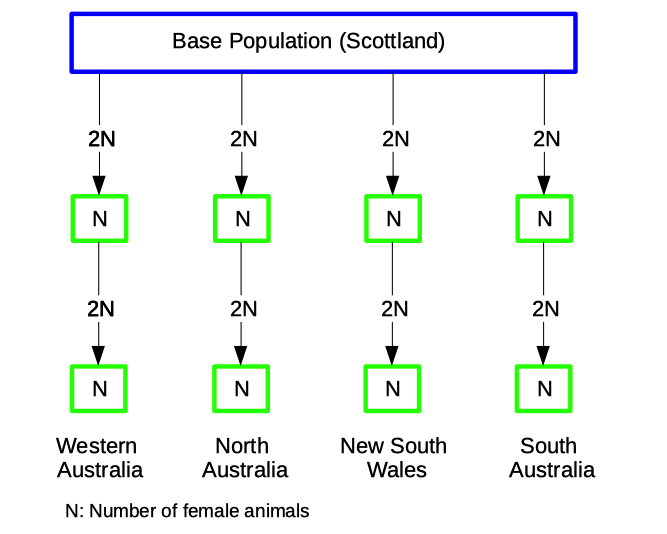
\includegraphics{odg/fig-sub-pop.png}

\vspace{3ex}

\begin{enumerate}
\item[a)] Compute the inbreeding coefficient $F_t$ for the breeding animals that the farmers want to sell. 

\textit{Berechnen Sie den Inzuchtkoeffizienten $F_t$ für die Zuchttiere, welche die Farmer verkaufen möchten.}
\points{4}
\end{enumerate}

\solstart

The inbreeding coefficient \(F_t\) is computed as

\[F_t = 1 - (1 - \Delta F)^t\] where \(\Delta F\) corresponds to
\(1/(2N)\) and \(t\) is equal to the number of generations. Inserting
the number leads to

\[F_t = 1 - (1 - 0.001)^{100} = 0.0952\]

\solend

\clearpage
\pagebreak

\begin{enumerate}
\item[b)] The sheep farmers are concerned that inbreeding in their population does not increase too much. In which year is the inbreeding coefficient $F_t$ going to be bigger than 0.1?

\textit{Die Farmer möchten den Inzuchtgrad nicht zu stark ansteigen lassen. In welchem Jahr wird der Inzuchtgrad $F_t$ grösser sein als 0.1?}
\points{2}
\end{enumerate}

\solstart

We are given the limit of \(F_t\) and we want to know the value for
\(t\) when this limit is reached. Hence we have to solve the equation
for \(F_t\) after \(t\). Hence

\begin{align}
F_t  &=  1 - (1 - \Delta F)^t \notag \\
(1 - \Delta F)^t  &=  1 - F_t \notag \\
t  &=  \frac{log(1 - F_t)}{log(1 - \Delta F)}  \notag \\
   &=  \frac{log(1 - 0.1)}{log(1 - 0.001)} = 105.3078266  \notag 
\end{align}

This means after 106 generations the limit is reached. With a generation
interval of 1.3 years, this will be the limit of the inbreeding
coefficient will be reached in the year 2030.

\solend

\clearpage
\pagebreak

\begin{enumerate}
\item[c)] One reason to control the inbreeding coefficient is that breeders want to avoid inbreeding depression. We assume that locus $W$ is mainly responsible for wool fibre diameter (FD). The favorable allele $W_1$ occurs with a frequency of $p = 0.045$. The difference between the homozygous genotypes $W_1W_1$ and $W_2W_2$ in fiber diameter is $100$ micrometer ($\mu m$). The genotypic value of the heterozygous genotype $W_1W_2$ is 15. Compute the inbreeding depression at locus $W$, if the inbreeding coefficient has reached the limiting value of Problem 1b of 0.1.

\textit{Züchter wollen die Inzucht begrenzen, da sie Inzuchtdepressionen vermeiden wollen. Wir nehmen an, dass das Merkmal Wollfaserdurchmesser hauptsächlich von einem Genort $W$ beeinflusst wird. Das vorteilhafte Allel $W_1$ kommt mit einer Häufigkeit von $p = 0.045$ vor. Die Differenz zwischen den homozygoten Genotypen $W_1W_1$ und $W_2W_2$ im Merkmal Wollfaserdurchmesser beträgt $100$ Mikrometer ($\mu m$). Der genotypische Wert der Heterozygoten $W_1W_2$ beträgt 15. Berechnen Sie die Inzuchtdepression am Genort $W$ unter der Annahme, dass der Inzuchtkoeffizient den Grenzwert aus Aufgabe 1b von 0.1 erreicht hat.}
\points{6}
\end{enumerate}

\vspace{3ex}
\solstart

The inbreeding depression is computed as

\[M_0 - M_F = 2d\bar{p}\bar{q}F = 2 * 15 * 0.045 * (1 -  0.045) * 0.1 =  0.1289\]

\solend

\clearpage
\pagebreak

\begin{enumerate}
\item[d)] Inbreeding has an influence on the genetic additive variance, as it is split into a between line and a within line component. Please, fill out the following table with the different genetic variance components for the locus $W$ from Problem 5c. We assume a value of  $0.1$ for the inbreeding coefficient $F$. 

\textit{Inzucht hat einen Einfluss auf die additive genetische Varianz, da diese Varianz durch die Inzucht in eine Komponente innerhalb Linie und eine Komponente zwischen Linien aufgeteilt wird. Bitte füllen Sie die folgende Tabelle mit den unterschiedlichen Varianzkomponenten am Genort $W$ aus Aufgabe 5c aus. Als Inzuchtkoeffizienten $F$ nehmen wir einen Wert von $0.1$ an.}
\points{10}
\end{enumerate}

\vspace{3ex}

\textbf{Solution}:

\begin{table}[H]
\centering
\begin{tabular}{l>{\raggedright\arraybackslash}p{8cm}}
\toprule
Source & Variance\\
\midrule
\begingroup\fontsize{12}{14}\selectfont Between lines\endgroup & \begingroup\fontsize{12}{14}\selectfont \endgroup\\
\begingroup\fontsize{12}{14}\selectfont Within lines\endgroup & \begingroup\fontsize{12}{14}\selectfont \endgroup\\
\begingroup\fontsize{12}{14}\selectfont Total additive\endgroup & \begingroup\fontsize{12}{14}\selectfont \endgroup\\
\begingroup\fontsize{12}{14}\selectfont Dominance\endgroup & \begingroup\fontsize{12}{14}\selectfont \endgroup\\
\begingroup\fontsize{12}{14}\selectfont Total genetic\endgroup & \begingroup\fontsize{12}{14}\selectfont \endgroup\\
\bottomrule
\end{tabular}
\end{table}

\vspace{3ex}
\solstart

\begin{table}[H]
\centering
\begin{tabular}{llr}
\toprule
Source & Variance & Values\\
\midrule
Between lines & $2FV_U$ & 42.98\\
Within lines & $(1-F)V_U$ & 193.39\\
Total additive & $(1+F)V_U$ & 236.36\\
Dominance & $V_D$ & 1.66\\
Total genetic & $V_G$ & 238.02\\
\bottomrule
\end{tabular}
\end{table}

\solend

\end{document}
